\chapter{线性规划}
\label{chap:opt-linear-programming}

一家作坊生产两种产品，每件分别获利$3$和$2$，两种原料每天各有$4$个单位，第一种产品每件消耗两种原料$2$和$1$个单位，第二种消耗$1$和$2$个单位。怎样安排产量才能获利最多？把所有允许的产量画在平面上，得到一个四边形；把“获利恰好等于某个数”的产量画出来，得到一族平行直线。让这条直线朝获利增加的方向平移，它最后离开四边形的位置是一个角点。这幅画面提出了本章要回答的几个问题：最优解为什么总能在角点中找到，角点很多时怎样不逐个枚举就走到最优的那个，怎样让别人不重复计算也能确认答案正确，问题无解或无界时又该交出什么。

目标和约束都是线性函数时，上面的几何直觉可以变成完整的计算。本章的学习目标，是在这类最具体的优化问题上走完一遍建模、求解和检验：把实际限制写成标准的线性模型，用线性方程组描述角点，用单纯形法沿边从一个角点走到相邻角点，再用对偶问题为“最优”“不可行”“无下界”三种结局分别给出可以独立核对的证书。得到一个解以后，还要回答两个改变对象不同的问题：数据变化时原来的解还能用多久，以及当原问题要求整数时，连续模型还能提供什么。

各节的先后由依赖关系决定。角点首先要有不依赖图形的定义，所以先写出模型并描述可行域的几何；把角点写成线性方程组的解之后，才能在角点之间设计计算。单纯形法停止时留下的数据恰好组成一组“资源价格”，它们给出最优值的界，证书因此从算法中自然产生；同一组价格又说明数据变化时最优值怎样变化。最后改变问题本身，研究要求整数的离散问题怎样借助线性规划获得界和候选。本章用到的凸集、凸组合、最优值与最优解等概念见第~\ref{chap:optimization}章。

\section{线性模型与可行域}
\label{sec:opt-lp-models}

章首的作坊问题用几句话就能说清，但要交给算法处理，必须先把“产量、获利、原料够不够”翻译成变量、目标和约束。本节先完成这一翻译，并把各种写法统一成一种便于计算的标准表示；随后研究全部可行候选组成的集合长什么样：它的边界由哪些约束决定，从一点出发可以朝哪些方向移动，它什么时候有角点，什么时候根本没有。

\subsection{线性规划的建模与标准型}
\label{sec:opt-lp-modeling}

\paragraph{从资源限制到线性模型}
设两种产品每天的产量分别为$x_1$和$x_2$。每件第一种产品获利$3$，每件第二种产品获利$2$，总获利是$3x_1+2x_2$。第一种原料每天有$4$个单位，两种产品每件分别消耗$2$和$1$个单位，所以产量必须满足$2x_1+x_2\le4$；第二种原料同样有$4$个单位，两种产品每件分别消耗$1$和$2$个单位，于是$x_1+2x_2\le4$。产量不能为负。把这些要求合在一起，得到
\begin{equation}
\label{eq:opt-lp-resource}
  \max_{x_1,x_2}\ 3x_1+2x_2
  \quad\text{s.t.}\quad
  2x_1+x_2\le4,\quad x_1+2x_2\le4,\quad x_1\ge0,\quad x_2\ge0.
\end{equation}
图~\ref{fig:opt-lp-resource-polygon}画出了它的全部可行产量：四条约束各切掉平面的一半，剩下的是以$(0,0)$、$(2,0)$、$(4/3,4/3)$、$(0,2)$为顶点的四边形。绿色直线是获利相同的产量，即目标的等值线$3x_1+2x_2=k$。$k$增大时，等值线沿方向$(3,2)$平行移动；$k=20/3$时它恰好只碰到顶点$(4/3,4/3)$，再增大就离开四边形。于是最大获利是$20/3$，在$x_1=x_2=4/3$处取得。本章后面的每一节都会回到这个例子。

\begin{figure}[!htbp]
  \centering
  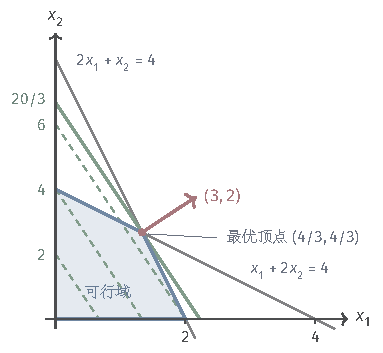
\includegraphics[width=64.904mm]{figures/03-optimization-evolution-and-signals/01-optimization/tikz/c2-resource-polygon/figure.pdf}
  \caption{资源分配例~\eqref{eq:opt-lp-resource}的可行域与目标等值线。浅蓝四边形是满足两条原料约束和非负约束的全部产量，两条灰线是原料恰好用完的边界。绿色虚线是获利为$2$、$4$、$6$的等值线，绿色实线是获利为$20/3$的等值线，纵轴左侧的绿色数字标出各条等值线的获利值；它们都与红色箭头$(3,2)$垂直，沿箭头平移时获利增大。获利$20/3$的等值线只在顶点$(4/3,4/3)$处碰到可行域。}
  \label{fig:opt-lp-resource-polygon}
\end{figure}

这个模型的特点在于目标和每一条约束都是变量的线性函数（可以带常数项）：获利按件数成比例累加，原料消耗也按件数成比例累加，两种产品之间没有相互作用。若生产第一种产品会使第二种产品的单位消耗打折，约束中就会出现$x_1x_2$这样的乘积项，模型不再是线性的。

\begin{definition}[线性规划]
\label{def:opt-lp-linear-program}
在$\mathbb R^n$中，以一个线性函数为目标，在有限个线性等式和非严格线性不等式约束下求最小值或最大值的问题，称为\term{线性规划}（linear programming, LP）。
\end{definition}

定义只允许非严格不等式。若允许$x_1<2$这样的严格不等式，可行域可能不包含它的边界点，最优值可能只能逼近而取不到；非严格不等式定义的可行域是闭集，这为后面最优解的存在性提供了条件。

\paragraph{整数要求不能直接放宽}
若产品只能按整件生产，就要再加上$x_1,x_2\in\mathbb Z$，得到的是\term{整数线性规划}（integer linear programming）。它的可行候选只是图~\ref{fig:opt-lp-resource-polygon}中四边形里的整数点$(0,0)$、$(1,0)$、$(2,0)$、$(0,1)$、$(1,1)$、$(0,2)$，逐个计算获利可知最优的是$(2,0)$，获利$6$。连续模型的解$(4/3,4/3)$不是整数；把它各坐标向下取整得到$(1,1)$，获利只有$5$。所以连续问题的最优解不能直接当作整数问题的解，二者的关系要另外研究，第~\ref{sec:opt-lp-relaxation}节专门处理这个问题。在此之前，本章讨论的都是变量取实数的线性规划。

\paragraph{标准型}
同一个线性规划可以有多种写法：求最大或最小，约束取“$\le$”“$\ge$”或“$=$”，变量有的要求非负，有的可正可负。为了用同一套公式计算，我们约定一种统一的写法。

\begin{definition}[线性规划的标准型]
\label{def:opt-lp-standard-form}
给定$\bm A\in\mathbb R^{m\times n}$、$\bm b\in\mathbb R^m$与$\bm c\in\mathbb R^n$，问题
\begin{equation}
\label{eq:opt-lp-standard}
  \min_{\bm x\in\mathbb R^n}\ \bm c^\top\bm x
  \quad\text{s.t.}\quad
  \bm A\bm x=\bm b,\quad \bm x\ge\bm 0
\end{equation}
称为线性规划的\term{标准型}（standard form），其中$\bm x\ge\bm 0$表示每个分量非负。记它的可行域为$P=\{\bm x\in\mathbb R^n:\bm A\bm x=\bm b,\ \bm x\ge\bm 0\}$。
\end{definition}

本章在讨论线性规划时把变量个数记为$n$、等式约束个数记为$m$，$\bm A$的第$j$列记为$\bm a_j$。下面逐项说明任意线性规划怎样改写成标准型，以及改写前后的解怎样相互恢复。

第一，最大化改为最小化：$\max\bm c^\top\bm x$与$\min(-\bm c)^\top\bm x$有相同的最优解，最优值互为相反数。第二，不等式改为等式：对约束$\bm g^\top\bm x\le h$，引入新变量$s=h-\bm g^\top\bm x$，约束等价于$\bm g^\top\bm x+s=h$且$s\ge0$，$s$称为\term{松弛变量}（slack variable），表示这条约束还剩多少余量；对$\bm g^\top\bm x\ge h$，则减去\term{剩余变量}（surplus variable）$s=\bm g^\top\bm x-h\ge0$。第三，可正可负的\term{自由变量}（free variable）$x_j$写成两个非负变量之差$x_j=x_j^+-x_j^-$。

这些变换保留的是“可行解之间的对应和目标值”，而不一定是一一对应。前两种变换中，新变量由原变量唯一确定，原问题的可行解与新问题的可行解一一对应，目标值不变。第三种变换中，从新问题的可行解总能恢复出$x_j=x_j^+-x_j^-$，目标值不变；但反过来同一个$x_j$有许多表示，例如$x_j=1$既可写成$(x_j^+,x_j^-)=(1,0)$，也可写成$(3,2)$。因此新问题的最优解可能不唯一，而它们都恢复为原问题的同一批最优解。

\begin{example}[资源模型的标准型]
\label{ex:opt-lp-resource-standard}
对模型~\eqref{eq:opt-lp-resource}，把目标改为最小化$-3x_1-2x_2$，并为两条原料约束引入松弛变量$x_3,x_4\ge0$，得到$n=4$、$m=2$的标准型
\[
  \bm A=\begin{pmatrix}2&1&1&0\\1&2&0&1\end{pmatrix},\qquad
  \bm b=\begin{pmatrix}4\\4\end{pmatrix},\qquad
  \bm c=(-3,-2,0,0)^\top.
\]
$x_3=4-2x_1-x_2$与$x_4=4-x_1-2x_2$分别是两种原料的剩余量。原问题的最优点$(4/3,4/3)$对应标准型中的$\bm x=(4/3,4/3,0,0)^\top$，两种原料恰好用完，目标值为$-20/3$。
\end{example}

\subsection{多面体、面与可行方向}
\label{sec:opt-lp-polyhedra}

图~\ref{fig:opt-lp-resource-polygon}中的四边形由四个半平面相交而成。高维情形无法画图，但“由有限个半空间相交”这一描述仍然成立，并足以推出可行域的主要几何性质。第~\ref{chap:optimization}章已经把有限个半空间的交称为多面体；本章统一写成
\[
  Q=\{\bm x\in\mathbb R^d:\bm G\bm x\le\bm h\}
  =\bigcap_{i=1}^k\{\bm x:\bm g_i^\top\bm x\le h_i\},
\]
其中$\bm G\in\mathbb R^{k\times d}$，$\bm h\in\mathbb R^k$，$\bm g_i^\top$是$\bm G$的第$i$行。

每个$\bm g_i\ne\bm 0$时，$\{\bm x:\bm g_i^\top\bm x\le h_i\}$是闭半空间，它的边界$\{\bm x:\bm g_i^\top\bm x=h_i\}$是仿射超平面；等式约束可以写成两个方向相反的不等式，所以有限个等式与不等式共同确定的集合仍是多面体。闭半空间是闭凸集，有限个闭凸集的交仍是闭凸集，所以多面体是闭凸集。标准型的可行域$P$也是多面体：它由$\bm A\bm x\le\bm b$、$-\bm A\bm x\le-\bm b$与$-\bm x\le\bm 0$确定。

\paragraph{活跃约束与面}
在多面体的一点$\bm x$处，有些约束恰好取等号，有些还留有余量。称$\bm g_i^\top\bm x=h_i$的约束为$\bm x$处的\term{活跃约束}（active constraint），记它们的指标集为$I(\bm x)=\{i:\bm g_i^\top\bm x=h_i\}$。对指标集$I\subseteq\{1,\dots,k\}$，令
\[
  F_I=\{\bm x\in Q:\bm g_i^\top\bm x=h_i,\ i\in I\}.
\]
非空的$F_I$称为$Q$的一个\term{面}（face）。取$I=\varnothing$得到$Q$本身；在图~\ref{fig:opt-lp-active-faces}的四边形中，让一条约束取等号得到一条边，让两条相交的约束同时取等号得到一个顶点。不同的指标集可能给出同一个面，例如在第~\ref{sec:opt-lp-degeneracy}节加入第三条过$(2,0)$的约束之后，任选其中两条取等号都得到同一个顶点。

\paragraph{可行方向}
站在可行域中的一点，哪些方向可以走一小步而不离开可行域？这由活跃约束决定。

\begin{definition}[可行方向]
\label{def:opt-lp-feasible-direction}
设$\bm x\in Q$，$\bm d\in\mathbb R^d$。若存在$\varepsilon>0$，使$\bm x+t\bm d\in Q$对全部$t\in[0,\varepsilon]$成立，就称$\bm d$是$Q$在$\bm x$处的\term{可行方向}（feasible direction）。
\end{definition}

\begin{lemma}[多面体的可行方向]
\label{lem:opt-lp-feasible-direction}
设$\bm x\in Q$。$\bm d$是$Q$在$\bm x$处的可行方向，当且仅当$\bm g_i^\top\bm d\le0$对每个$i\in I(\bm x)$成立。
\end{lemma}

\begin{proof}
若某个$i\in I(\bm x)$满足$\bm g_i^\top\bm d>0$，则对任意$t>0$有$\bm g_i^\top(\bm x+t\bm d)=h_i+t\bm g_i^\top\bm d>h_i$，所以$\bm d$不是可行方向。反过来，设全部活跃约束都满足$\bm g_i^\top\bm d\le0$。对活跃约束，$\bm g_i^\top(\bm x+t\bm d)\le h_i$对所有$t\ge0$成立。不活跃的约束有余量$h_i-\bm g_i^\top\bm x>0$；若$\bm g_i^\top\bm d\le0$，它对所有$t\ge0$都成立，否则只要$t\le(h_i-\bm g_i^\top\bm x)/\bm g_i^\top\bm d$就仍成立。不活跃约束只有有限条，取这些正上界中的最小值作为$\varepsilon$（没有正上界时取$\varepsilon=1$）即可。
\end{proof}

引理把“能否移动”变成了只看活跃约束的有限个线性不等式。图~\ref{fig:opt-lp-active-faces}画出了三种典型位置。内部点没有活跃约束，任何方向都可以走；边上的点只有一条活跃约束，例如在边$2x_1+x_2=4$上，可行方向是满足$2d_1+d_2\le0$的半平面；在顶点$(4/3,4/3)$处两条约束同时活跃，可行方向是同时满足$2d_1+d_2\le0$与$d_1+2d_2\le0$的锥，它由$(1,-2)$和$(-2,1)$两个边方向张成，正好指向可行域内部。活跃约束越多，能走的方向越少。

\begin{figure}[!htbp]
  \centering
  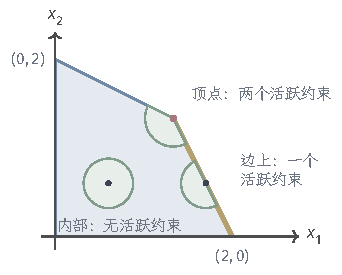
\includegraphics[width=57.993mm]{figures/03-optimization-evolution-and-signals/01-optimization/tikz/c2-active-faces/figure.pdf}
  \caption{活跃约束与可行方向。在资源分配例的可行域中，绿色区域表示从黑点或红点出发可以走一小步的方向：内部点处是整个圆盘，边上的点处是半个圆盘，顶点$(4/3,4/3)$处是两条边方向张成的锥。黄色粗线是约束$2x_1+x_2\le4$取等号得到的面，即一条边。}
  \label{fig:opt-lp-active-faces}
\end{figure}

\paragraph{极点}
顶点在图中一眼就能认出，但高维时需要一个不依赖图形的定义。观察图~\ref{fig:opt-lp-active-faces}：内部点和边上的点都位于某条可行线段的中间，顶点却不是任何两个不同可行点连线的中间点。

\begin{definition}[极点]
\label{def:opt-lp-extreme-point}
设$C$是凸集，$\bm x\in C$。若$\bm x=\lambda\bm u+(1-\lambda)\bm v$、$\bm u,\bm v\in C$、$\lambda\in(0,1)$总推出$\bm u=\bm v=\bm x$，就称$\bm x$是$C$的\term{极点}（extreme point）。
\end{definition}

在二维例子中，极点恰好是两条线性无关的约束同时取等号的点。下一节将在标准型中证明相应的一般结论：极点就是可以由一个线性方程组解出的“基本可行解”。

\paragraph{空集、有界与无界}
多面体可以有几种很不相同的形状，图~\ref{fig:opt-lp-polyhedron-cases}列出了与线性规划有关的几种。约束彼此矛盾时多面体是空集，例如在第一象限中同时要求$x_1+x_2\le1$与$x_1+x_2\ge2$。多面体也可以无界。若$Q$非空，且方向$\bm d$满足$\bm G\bm d\le\bm 0$，则对任意$\bm x\in Q$和$t\ge0$都有$\bm G(\bm x+t\bm d)\le\bm h$，即沿$\bm d$可以一直走下去而不离开$Q$；这样的$\bm d$称为$Q$的\term{回收方向}（recession direction）。

可行域无界并不意味着目标无下界。图~\ref{fig:opt-lp-polyhedron-cases}(b)与(c)用的是同一个无界区域$\{x_1\ge0,\ x_2\ge0,\ x_1+x_2\ge1\}$。最小化$x_1+2x_2$时，所有回收方向$\bm d\ge\bm 0$都使目标不减，最小值$1$在$(1,0)$处达到；最小化$x_2-x_1$时，沿回收方向$\bm d=(1,0)$走$t$步，目标减少$t$，所以没有下界。决定目标有无下界的是目标沿回收方向的变化，而不是可行域是否有界。反过来，若可行域非空且有界，它是$\mathbb R^d$中的有界闭集，连续的线性目标一定能取到最小值。

\begin{figure*}[!htbp]
  \centering
  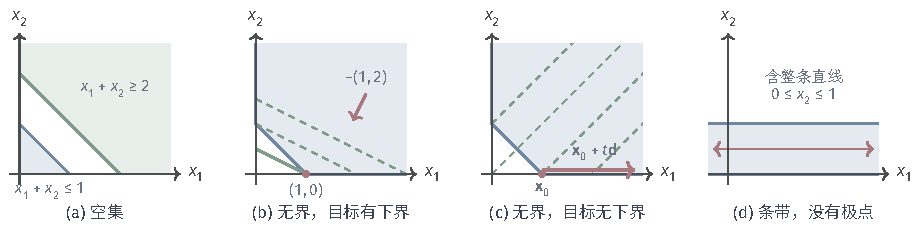
\includegraphics[width=156.496mm]{figures/03-optimization-evolution-and-signals/01-optimization/tikz/c2-polyhedron-cases/figure.pdf}
  \caption{几种多面体。(a) 第一象限中$x_1+x_2\le1$的部分（蓝）与$x_1+x_2\ge2$的部分（绿）不相交，多面体为空集。(b) 无界区域$\{x_1,x_2\ge0,\ x_1+x_2\ge1\}$上最小化$x_1+2x_2$，绿色线为等值线，红色箭头是目标下降的方向，最小值$1$在$(1,0)$处达到。(c) 同一区域上最小化$x_2-x_1$，从$\bm x_0=(1,0)$沿$\bm d=(1,0)$前进，目标无限下降。(d) 条带$0\le x_2\le1$（$x_1$不受限制）包含整条水平直线，没有极点。}
  \label{fig:opt-lp-polyhedron-cases}
\end{figure*}

\paragraph{直线、条带与最优面}
多面体还可能根本没有极点。图~\ref{fig:opt-lp-polyhedron-cases}(d)的条带$\{(x_1,x_2):0\le x_2\le1\}$对每个点都包含一整条水平直线：任何点都是左右两个可行点的中点，所以没有极点。直线$\{(x_1,0):x_1\in\mathbb R\}$本身也是多面体，同样没有极点。在这样的区域上最小化$x_2$，最小值$0$在整条直线上取得，却没有一个“角点”可以代表它。

标准型的可行域$P$不会出现这种情况。若$\bm x+t\bm d\in P$对全部实数$t$成立，则每个坐标$x_j+td_j$对正负两个方向的$t$都非负，只能有$d_j=0$；所以$P$不包含任何直线。下一节正是利用这一点证明：非空的$P$一定有极点，并且有限的最优值一定能在某个极点处取得。这也是我们选择标准型作为计算对象的一个理由。

最后，最优解不一定唯一。若目标的等值线恰好与可行域的一条边平行，在等值线平移到最后时，它接触的是整条边，边上每一点都是最优解，例如图~\ref{fig:opt-lp-optimal-face}(b)。全部最优解组成的集合$\{\bm x\in Q:\bm c^\top\bm x=f^\star\}$称为\term{最优面}（optimal face），其中$f^\star$是最优值；它是凸集；对标准型，第~\ref{sec:opt-lp-strong-duality}节会说明它确实是可行域的一个面。从图形上看到等值线接触到可行域，只能说明找到了最优值，不能据此断言最优解唯一。

\section{基本可行解与最优解}
\label{sec:opt-lp-basic-solutions}

在平面上，顶点是两条边界直线的交点，求它只需解一个二元一次方程组。标准型~\eqref{eq:opt-lp-standard}生活在$\mathbb R^n$中，有$m$个等式；若再让$n-m$个坐标取零，剩下$m$个未知数、$m$个方程，一般也能解出唯一一点。本节把这一观察整理成“基”和“基本可行解”，证明它们恰好是可行域的极点，并证明只要最优值有限，就能在有限个基本可行解中找到最优解。这为单纯形法在基之间组织搜索提供了依据。

\subsection{基、基本解与基本可行解}
\label{sec:opt-lp-bases}

\paragraph{满行秩假设}
用“选$m$列解方程”来描述点之前，先要保证等式系统没有多余的方程。由线性方程的解结构，$\bm A\bm x=\bm b$有解当且仅当$\operatorname{rank}\bm A=\operatorname{rank}[\bm A\ \bm b]$；有解时，若$\operatorname{rank}\bm A=r<m$，可以挑出$r$个线性无关的行，其余各行都是它们的线性组合，删去其余行不改变解集。这里用到的秩判别、消元与LU分解，可参考\BookChapterRef{chap:linear-equations-and-optimization}{卷一“线性方程与矩阵方程”章}。若方程不相容，可行域是空集，问题已经回答。因此在讨论基之前，我们总假设$\bm A\in\mathbb R^{m\times n}$满行秩，即$\operatorname{rank}\bm A=m\le n$。实际计算中并不需要预先做这一步，第~\ref{sec:opt-lp-two-phase}节的第一阶段会在求可行点的同时发现冗余行。

\begin{definition}[基与基本可行解]
\label{def:opt-lp-basic-feasible}
设$\bm A$满行秩。若$m$个指标组成的集合$B\subseteq\{1,\dots,n\}$使对应各列构成的方阵$\bm A_B$可逆，就称$B$为一个基，$\bm A_B$为\term{基矩阵}（basis matrix），其余指标记为$N$。令$\bm x_N=\bm 0$，并由$\bm A_B\bm x_B=\bm b$解出$\bm x_B=\bm A_B^{-1}\bm b$，所得的$\bm x$称为基$B$对应的\term{基本解}（basic solution）；$x_j$（$j\in B$）称为\term{基变量}（basic variable），$x_j$（$j\in N$）称为\term{非基变量}（nonbasic variable）。若还有$\bm x_B\ge\bm 0$，就称$\bm x$为\term{基本可行解}（basic feasible solution）。若某个基变量取零，称这个基本可行解是退化的。
\end{definition}

基本解满足全部等式，但不一定满足非负约束；只有$\bm x_B\ge\bm 0$时它才落在可行域中。

\begin{example}[资源模型的六个基本解]
\label{ex:opt-lp-six-basic-solutions}
在例~\ref{ex:opt-lp-resource-standard}中$m=2$、$n=4$，四列中任取两列都线性无关，共有$\binom42=6$个基。以$B=\{1,4\}$为例，令$x_2=x_3=0$，方程组变为$2x_1=4$、$x_1+x_4=4$，解得$x_1=2$、$x_4=2$，对应平面上的点$(2,0)$，第二种原料还剩$2$个单位。同样算得：$B=\{3,4\}$给出$(0,0)$，$B=\{2,3\}$给出$(0,2)$，$B=\{1,2\}$给出$(4/3,4/3)$，这四个是基本可行解。$B=\{1,3\}$令$x_2=x_4=0$，第二个方程给出$x_1=4$，第一个方程给出$x_3=4-8=-4<0$，基本解$(4,0)$用掉的第一种原料超过库存；$B=\{2,4\}$类似地给出$(0,4)$与$x_4=-4$。图~\ref{fig:opt-lp-basic-solutions}把六个基本解画在平面上：它们正是四条边界直线两两的交点，其中落在四边形上的四个恰好是四个顶点。
\end{example}

\begin{figure}[!htbp]
  \centering
  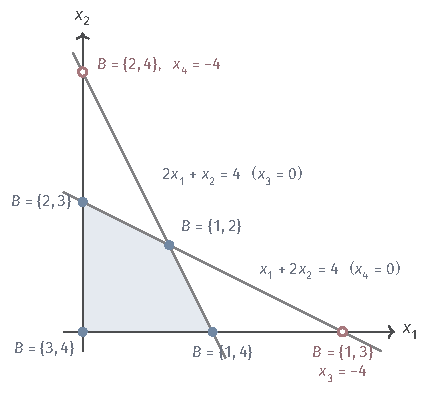
\includegraphics[width=72.796mm]{figures/03-optimization-evolution-and-signals/01-optimization/tikz/c2-basic-solutions/figure.pdf}
  \caption{资源分配例的六个基本解。每个基$B$指定两个取正值的候选变量，其余两个变量取零，即令两条边界同时取等号；$x_3=0$与$x_4=0$分别对应两条灰线，$x_1=0$与$x_2=0$对应两条坐标轴。蓝色实心点是四个基本可行解，即可行域的四个顶点；红色空心点是两个基本解，它们各有一个松弛变量为负，落在可行域外。}
  \label{fig:opt-lp-basic-solutions}
\end{figure}

\paragraph{退化：多个基，同一个点}
基与点不一定一一对应。在资源模型中再加一条市场限制$x_1\le2$，引入松弛变量$x_5$，得到$m=3$、$n=5$的标准型。可行域没有变化，因为$x_1\le2$在原四边形上本来就成立；但顶点$(2,0)$现在有三条边界同时经过：$x_2=0$、$2x_1+x_2=4$与$x_1=2$。这一点对应的$\bm x=(2,0,0,2,0)^\top$只有$x_1$和$x_4$两个正分量，而基要有三个指标。把第三个指标取为$3$、$5$或$2$都能使基矩阵可逆，三个基$\{1,3,4\}$、$\{1,4,5\}$、$\{1,2,4\}$给出同一个点，每个基中都有一个取零的基变量。所以“基变量的个数”$m$与“正分量的个数”不必相同，后者可以更少。第~\ref{sec:opt-lp-degeneracy}节会看到，这种退化会让单纯形法换了基却停在原地。

\paragraph{基本可行解就是极点}
下面的定理把代数对象（基本可行解）与几何对象（极点）连起来，并给出一个不需要先找基的判别：只看正分量所在的列。

\begin{theorem}[基本可行解与极点]
\label{thm:opt-lp-bfs-extreme}
设$\bm A$满行秩，$\bm x\in P$，记$J=\{j:x_j>0\}$。以下三条等价：
\begin{enumerate}
  \item $\bm x$是$P$的极点；
  \item 列$\{\bm a_j:j\in J\}$线性无关；
  \item $\bm x$是某个基对应的基本可行解。
\end{enumerate}
\end{theorem}

\begin{proof}
(1)$\Rightarrow$(2)：若这些列线性相关，存在不全为零的系数$w_j$（$j\in J$）使$\sum_{j\in J}w_j\bm a_j=\bm 0$。把$\bm w$在$J$以外的分量补为零，就有$\bm A\bm w=\bm 0$且$\bm w\ne\bm 0$。由于$x_j>0$对$j\in J$成立，取足够小的$\varepsilon>0$可使$\bm x\pm\varepsilon\bm w\ge\bm 0$，又$\bm A(\bm x\pm\varepsilon\bm w)=\bm b$，所以$\bm x\pm\varepsilon\bm w$都可行，且它们不相等，$\bm x$是二者的中点。这与$\bm x$是极点矛盾。

(2)$\Rightarrow$(3)：线性无关的列至多$m$个，所以$|J|\le m$。$\bm A$满行秩，它的列张成$\mathbb R^m$，可以从其余列中补进若干列，把$\{\bm a_j:j\in J\}$扩充为$\mathbb R^m$的一组基，相应指标集记为$B\supseteq J$。于是$\bm A_B$可逆，$N=\{1,\dots,n\}\setminus B$中的指标都不在$J$中，$\bm x_N=\bm 0$；再由$\bm A\bm x=\bm A_B\bm x_B=\bm b$得$\bm x_B=\bm A_B^{-1}\bm b$。$\bm x$可行，故$\bm x_B\ge\bm 0$，它是基$B$的基本可行解。

(3)$\Rightarrow$(1)：设$\bm x$是基$B$的基本可行解，且$\bm x=\lambda\bm u+(1-\lambda)\bm v$，$\bm u,\bm v\in P$，$\lambda\in(0,1)$。对$j\in N$，$0=x_j=\lambda u_j+(1-\lambda)v_j$，而$u_j,v_j\ge0$，只能$u_j=v_j=0$。于是$\bm A_B\bm u_B=\bm b$，$\bm u_B=\bm A_B^{-1}\bm b=\bm x_B$，即$\bm u=\bm x$；同理$\bm v=\bm x$。所以$\bm x$是极点。
\end{proof}

证明的第一步给出了一个今后反复使用的操作：若可行点的正分量所在列线性相关，就能找到方向$\bm w\ne\bm 0$，满足$\bm A\bm w=\bm 0$且只在正分量上非零，沿$\pm\bm w$都能走一小段而不离开可行域。定理也提醒我们，“手里有一个可行点”与“手里有一个可用的基”是两回事：一般可行点的正分量可能多于$m$个，它不是基本可行解，要从它得到一个基还需要计算。

\subsection{最优基本可行解与最优面}
\label{sec:opt-lp-optimal-bfs}

图~\ref{fig:opt-lp-resource-polygon}中最优解落在顶点上。下面证明这在标准型中总成立：只要可行域非空、目标有下界，就存在作为基本可行解的最优解。证明不预先假设最优解存在，而是把任意可行点“推”到一个不更差的基本可行解上。

\begin{lemma}[推向基本可行解]
\label{lem:opt-lp-push-to-bfs}
设$\bm A$满行秩，$P\ne\varnothing$，且$\bm c^\top\bm x$在$P$上有下界。则对每个$\bm x\in P$，存在基本可行解$\widehat{\bm x}$，使$\bm c^\top\widehat{\bm x}\le\bm c^\top\bm x$。
\end{lemma}

\begin{proof}
对正分量个数$|J|$（$J=\{j:x_j>0\}$）作归纳。若列$\{\bm a_j:j\in J\}$线性无关，由定理~\ref{thm:opt-lp-bfs-extreme}，$\bm x$本身是基本可行解。否则，像定理证明中那样取$\bm w\ne\bm 0$，满足$\bm A\bm w=\bm 0$且$w_j=0$对$j\notin J$成立。必要时把$\bm w$换成$-\bm w$，可使$\bm c^\top\bm w\le0$。

先排除一种情形：$\bm c^\top\bm w<0$且$\bm w\ge\bm 0$。此时对一切$t\ge0$，$\bm x+t\bm w\ge\bm 0$且$\bm A(\bm x+t\bm w)=\bm b$，目标值$\bm c^\top\bm x+t\bm c^\top\bm w$随$t$趋于$-\infty$，与有下界矛盾。若$\bm c^\top\bm w=0$且$\bm w\ge\bm 0$，则把$\bm w$换成$-\bm w$，仍有$\bm c^\top\bm w=0\le0$，而且$-\bm w$有负分量。因此总可以假设$\bm c^\top\bm w\le0$，并且$\bm w$至少有一个负分量。

令
\[
  t^\star=\min\Bigl\{\frac{x_j}{-w_j}:w_j<0\Bigr\}>0,\qquad
  \bm x'=\bm x+t^\star\bm w.
\]
$t^\star$的取法保证$\bm x'\ge\bm 0$，又$\bm A\bm x'=\bm b$，所以$\bm x'\in P$，且$\bm c^\top\bm x'=\bm c^\top\bm x+t^\star\bm c^\top\bm w\le\bm c^\top\bm x$。$\bm w$只在$J$上非零，$J$以外的分量保持为零，而取到最小值的那个分量变为零，所以$\bm x'$的正分量个数严格减少。由归纳假设，$\bm x'$可以推到一个基本可行解$\widehat{\bm x}$，$\bm c^\top\widehat{\bm x}\le\bm c^\top\bm x'\le\bm c^\top\bm x$。
\end{proof}

\begin{theorem}[最优基本可行解的存在性]
\label{thm:opt-lp-optimal-bfs}
设$\bm A$满行秩。若标准型~\eqref{eq:opt-lp-standard}可行且目标在$P$上有下界，则最优值能够取到，并且至少有一个最优解是基本可行解。特别地，非空的$P$至少有一个极点。
\end{theorem}

\begin{proof}
基至多有$\binom nm$个，所以基本可行解只有有限个；对$P$中任一点应用引理~\ref{lem:opt-lp-push-to-bfs}，知它们至少有一个。在有限个基本可行解中取目标值最小的$\bm x^\star$。对任意$\bm x\in P$，引理给出基本可行解$\widehat{\bm x}$，使$\bm c^\top\bm x\ge\bm c^\top\widehat{\bm x}\ge\bm c^\top\bm x^\star$。所以$\bm x^\star$是全局最优解。最后一句取$\bm c=\bm 0$即得。
\end{proof}

这个定理是线性规划区别于一般优化问题的地方：一般问题中“有下界”推不出“下确界能取到”，例如$e^{x}$在$\mathbb R$上有下界$0$却取不到；在标准型线性规划中，有限的最优值总能取到。证明用到了两点：$\bm x\ge\bm 0$使可行域不含直线，引理中总有一个分量会先降到零；线性目标沿直线的变化是线性的，要么能朝不变差的方向推进，要么出现无下界的射线。

\paragraph{枚举基的代价}
定理说明，原则上可以列出全部基，解出基本解，丢掉不可行的，再比较目标值。资源模型只有$6$个基，这样做毫无困难。但基的个数$\binom nm$随规模急剧增长：$n=100$、$m=50$时约为$1.0\times10^{29}$。即使每秒检查$10^{12}$个基，也远远无法完成。我们需要只在“相邻”的基之间移动、并且每一步都让目标不变差的方法，这就是下一节的单纯形法。

\paragraph{最优解未必都是基本可行解}
定理只断言存在一个最优的基本可行解，并不是说每个最优解都是基本可行解。图~\ref{fig:opt-lp-optimal-face}比较了同一可行域上的两个目标。最大化$3x_1+2x_2$时，最优解只有顶点$(4/3,4/3)$。改为最大化$2x_1+x_2$时，目标等值线与边$2x_1+x_2=4$平行，最优值为$4$，两个顶点$(2,0)$与$(4/3,4/3)$都最优，它们的连线上每一点也都最优。例如二者的中点$(5/3,2/3)$对应标准型中的$\bm x=(5/3,2/3,0,1)^\top$，有三个正分量，多于$m=2$，所以它不是基本可行解，却同样最优。这里的最优面是两个最优顶点的全部凸组合，即一整条边。因此，若求解方法只报告一个顶点，它回答了“最优值是多少”和“一个最优解是什么”，并没有回答“最优解是否唯一”。

\begin{figure}[!htbp]
  \centering
  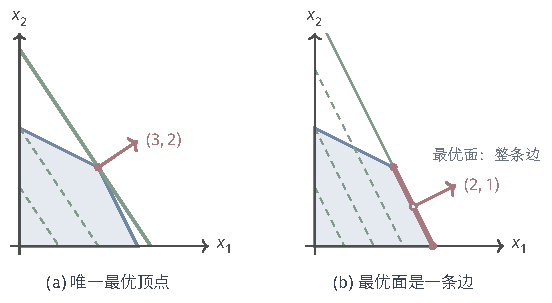
\includegraphics[width=93.419mm]{figures/03-optimization-evolution-and-signals/01-optimization/tikz/c2-optimal-face/figure.pdf}
  \caption{同一可行域上的唯一最优解与多个最优解。(a) 最大化$3x_1+2x_2$，绿色实线为最优等值线$3x_1+2x_2=20/3$，它只接触顶点$(4/3,4/3)$。(b) 最大化$2x_1+x_2$，绿色虚线为等值线$2x_1+x_2=1,2,3$，最优等值线$2x_1+x_2=4$与一条边重合；红色粗线上的点都最优，空心点$(5/3,2/3)$是其中一个不是顶点的最优解。}
  \label{fig:opt-lp-optimal-face}
\end{figure}

\section{单纯形法}
\label{sec:opt-lp-simplex}

上一节说明最优解可以在有限个基本可行解中寻找，但不能逐个枚举。单纯形法的想法来自图~\ref{fig:opt-lp-resource-polygon}：站在一个顶点上，检查从它出发的各条边，若某条边能让目标下降，就沿这条边走到下一个顶点；若没有这样的边，就停下。本节把这三步翻译成线性代数：怎样在当前基下判断哪条边下降、走多远、走到哪个新基；随后补上算法还缺的三块——第一个可行基从哪里来，退化时怎样避免原地打转，以及在计算机上怎样稳定、省力地实现这些更新。

\subsection{约化费用与换基更新}
\label{sec:opt-lp-reduced-cost}

\paragraph{用非基变量表示目标}
设$B$是一个可行基，当前基本可行解为$\bm x$。对任意满足$\bm A\bm x=\bm b$的点，把等式拆成基部分与非基部分，$\bm A_B\bm x_B+\bm A_N\bm x_N=\bm b$，于是基变量完全由非基变量决定：
\[
  \bm x_B=\bm A_B^{-1}(\bm b-\bm A_N\bm x_N).
\]
代入目标$\bm c^\top\bm x=\bm c_B^\top\bm x_B+\bm c_N^\top\bm x_N$，得到
\begin{equation}
\label{eq:opt-lp-reduced-cost}
  \bm c^\top\bm x=\bm c_B^\top\bm A_B^{-1}\bm b+\bar{\bm c}_N^\top\bm x_N,
  \qquad
  \bar{\bm c}_N=\bm c_N-\bm A_N^\top\bm A_B^{-\top}\bm c_B.
\end{equation}
第一项是当前顶点的目标值，第二项说明：让非基变量$x_j$从零增加一个单位，目标改变$\bar c_j$。$\bar c_j$称为$x_j$的\term{约化费用}（reduced cost）。记$\bm y=\bm A_B^{-\top}\bm c_B\in\mathbb R^m$，则$\bar c_j=c_j-\bm a_j^\top\bm y$，对基变量同样定义，有$\bar c_j=0$（$j\in B$）。$\bm y$的含义将在第~\ref{sec:opt-lp-duality}节揭晓，这里先把它看作计算约化费用的中间量。

\begin{theorem}[最优性判别]
\label{thm:opt-lp-optimality-criterion}
若可行基$B$的约化费用满足$\bar{\bm c}_N\ge\bm 0$，则它的基本可行解是标准型~\eqref{eq:opt-lp-standard}的全局最优解。
\end{theorem}

\begin{proof}
任取可行点$\bm x'$。它满足$\bm A\bm x'=\bm b$，所以式~\eqref{eq:opt-lp-reduced-cost}对它成立；又$\bm x'_N\ge\bm 0$，故$\bm c^\top\bm x'=\bm c_B^\top\bm A_B^{-1}\bm b+\bar{\bm c}_N^\top\bm x'_N\ge\bm c_B^\top\bm A_B^{-1}\bm b$，右端正是当前基本可行解的目标值。
\end{proof}

判别只比较当前顶点与它相邻的边，结论却是全局的，原因是式~\eqref{eq:opt-lp-reduced-cost}对全部可行点成立，而可行点的非基分量都非负。反过来，若某个$\bar c_j<0$，并不总能断定当前点不是最优：在退化的基下，沿这条边可能一步也走不动（第~\ref{sec:opt-lp-degeneracy}节）。基本可行解非退化时，下面的计算会说明沿这条边确实能使目标严格下降。

\paragraph{沿一条边移动}
选一个$\bar c_j<0$的非基变量$x_j$，称为\term{入基变量}（entering variable）。让$x_j$从$0$增加到$\theta\ge0$，其余非基变量保持为零，基变量随之调整以保持等式成立。由上式，$\bm x_B(\theta)=\bm x_B-\theta\bm A_B^{-1}\bm a_j$。把这一移动写成$\bm x(\theta)=\bm x+\theta\bm d$，方向$\bm d$满足
\begin{equation}
\label{eq:opt-lp-direction}
  d_j=1,\qquad d_k=0\ (k\in N,\ k\ne j),\qquad \bm d_B=-\bm A_B^{-1}\bm a_j.
\end{equation}
直接验证$\bm A\bm d=\bm a_j+\bm A_B\bm d_B=\bm 0$，所以沿$\bm d$移动始终满足等式；目标沿$\bm d$的变化率是$\bm c^\top\bm d=c_j-\bm c_B^\top\bm A_B^{-1}\bm a_j=\bar c_j<0$。在图上，这就是从当前顶点出发、沿一条边离开的方向。

\paragraph{最小比值检验}
沿$\bm d$能走多远，取决于基变量何时降到零。$d_i\ge0$的基变量不会减小；$d_i<0$的基变量在$\theta=x_i/(-d_i)$时降到零。为了保持非负，步长取
\begin{equation}
\label{eq:opt-lp-ratio-test}
  \theta^\star=\min\Bigl\{\frac{x_i}{-d_i}:i\in B,\ d_i<0\Bigr\}.
\end{equation}
这称为\term{最小比值检验}（minimum ratio test）。达到最小值的基变量$x_\ell$首先降到零，称为\term{出基变量}（leaving variable）。若所有$d_i\ge0$，则$\bm x+\theta\bm d$对一切$\theta\ge0$都可行，目标以速率$\bar c_j<0$无限下降，问题无下界，$\bm x$与$\bm d$一起就是这一结论的证据。

\begin{lemma}[换基]
\label{lem:opt-lp-pivot}
设$d_\ell<0$且$\ell$在式~\eqref{eq:opt-lp-ratio-test}中达到最小值。则$B'=(B\setminus\{\ell\})\cup\{j\}$仍是一个基，$\bm x(\theta^\star)$是它的基本可行解，目标值为$\bm c^\top\bm x+\theta^\star\bar c_j$。
\end{lemma}

\begin{proof}
$\bm A_B\bm d_B=-\bm a_j$说明$\bm a_j$用基列表示时，$\bm a_\ell$的系数是$-d_\ell\ne0$。若$B'$的列线性相关，$\bm a_j$就能由$B\setminus\{\ell\}$的列表示，这与表示的唯一性及该系数非零矛盾，所以$\bm A_{B'}$可逆。$\theta^\star$的取法保证$\bm x(\theta^\star)\ge\bm 0$，等式由$\bm A\bm d=\bm 0$保持；它的分量$x_\ell(\theta^\star)=0$，在$N\setminus\{j\}$上的分量也为零，即$B'$以外的分量都为零，所以它就是$B'$的基本可行解。目标值由$\bm c^\top\bm d=\bar c_j$得到。
\end{proof}

用一个新指标替换一个旧指标、从一个基转到相邻的基，称为\term{换基}（pivoting）。几何上，新基本可行解是沿边走到的下一个顶点。$\theta^\star>0$时目标严格下降$\theta^\star|\bar c_j|$；$\theta^\star=0$只可能在当前解退化（某个$x_\ell=0$且$d_\ell<0$）时发生。下面把这些步骤合成算法；初始可行基和出入基的选取规则分别在后两小节给出。

\begin{algorithm}[单纯形法（给定可行基）]
\label{alg:opt-lp-simplex}
\begin{algorithmic}[1]
\Require 满行秩的$\bm A\in\mathbb R^{m\times n}$，$\bm b$，$\bm c$；可行基$B$，即$\bm A_B^{-1}\bm b\ge\bm 0$
\Ensure 最优基本可行解$\bm x$及乘子$\bm y$；或可行点$\bm x$及无下界方向$\bm d$
\Loop
  \State 解$\bm A_B\bm x_B=\bm b$，令$\bm x_N=\bm 0$
  \State 解$\bm A_B^\top\bm y=\bm c_B$，对$j\in N$计算$\bar c_j=c_j-\bm a_j^\top\bm y$
  \If{$\bar c_j\ge0$对全部$j\in N$成立}
    \State \Return 最优解$\bm x$与$\bm y$
  \EndIf
  \State 按入基规则选一个$\bar c_j<0$的$j$
  \State 解$\bm A_B\bm u=\bm a_j$，按式~\eqref{eq:opt-lp-direction}令$\bm d_B=-\bm u$
  \If{$\bm d_B\ge\bm 0$}
    \State \Return 可行点$\bm x$与方向$\bm d$ \Comment{$\bm A\bm d=\bm 0$，$\bm d\ge\bm 0$，$\bm c^\top\bm d<0$}
  \EndIf
  \State 按式~\eqref{eq:opt-lp-ratio-test}求$\theta^\star$，按出基规则选达到最小值的$\ell$
  \State $B\gets(B\setminus\{\ell\})\cup\{j\}$
\EndLoop
\end{algorithmic}
\end{algorithm}

算法每轮的主要工作是两个$m$阶线性方程组和对非基列的定价。入基规则若取约化费用最负的那个，就是最常见的Dantzig规则；它只是一种经验选择，不保证轮数最少。

\paragraph{手算一次}
对资源模型的标准型（例~\ref{ex:opt-lp-resource-standard}），松弛变量提供了现成的可行基$B=\{3,4\}$：$\bm A_B=\bm I$，基本可行解是原点，$x_3=x_4=4$。表~\ref{tab:opt-lp-simplex-run}记录了每一轮的数据。

第$0$轮，$\bm c_B=\bm 0$，所以$\bm y=\bm 0$，约化费用就是$\bar c_1=-3$、$\bar c_2=-2$：两种产品都还没生产，生产任何一种都能增加获利。按Dantzig规则让$x_1$入基。$\bm u=\bm A_B^{-1}\bm a_1=(2,1)^\top$，即$x_1$每增加一单位，$x_3$减少$2$、$x_4$减少$1$；比值为$4/2=2$与$4/1=4$，所以$\theta^\star=2$，$x_3$出基。图~\ref{fig:opt-lp-simplex-path}(b)把这一检验画成了直线：$x_3=4-2\theta$先撞到零，再往前走第一种原料就不够了。新顶点是$(2,0)$，目标值$-6$。

第$1$轮，$B=\{1,4\}$。解$\bm A_B^\top\bm y=\bm c_B$，即$2y_1+y_2=-3$、$y_2=0$，得$\bm y=(-3/2,0)^\top$。于是$\bar c_2=-2-(1\cdot(-3/2)+2\cdot0)=-1/2$，$\bar c_3=0-(-3/2)=3/2$。$x_2$入基；解$\bm A_B\bm u=\bm a_2$，即$2u_1=1$、$u_1+u_4=2$，得$\bm u=(1/2,3/2)^\top$，即$x_2$每增加一单位，$x_1$减少$1/2$、$x_4$减少$3/2$。比值为$2/(1/2)=4$与$2/(3/2)=4/3$，$\theta^\star=4/3$，$x_4$出基。新顶点$(4/3,4/3)$，目标值$-6+(4/3)(-1/2)=-20/3$。

第$2$轮，$B=\{1,2\}$。解$2y_1+y_2=-3$、$y_1+2y_2=-2$，得$\bm y=(-4/3,-1/3)^\top$，$\bar c_3=4/3$、$\bar c_4=1/3$，全部非负。由定理~\ref{thm:opt-lp-optimality-criterion}，$(4/3,4/3)$最优，与图解一致。若第$0$轮改让$x_2$入基，路径会经过另一个顶点$(0,2)$，同样两轮到达最优，见图~\ref{fig:opt-lp-simplex-path}(a)中的虚线。

\begin{table*}[!htbp]
  \centering
  \caption{资源模型上的单纯形法。每轮列出当前基、基本可行解、乘子$\bm y=\bm A_B^{-\top}\bm c_B$、非基变量的约化费用、换基选择与目标值$\bm c^\top\bm x$；最后一轮约化费用全部非负，算法停止。}
  \label{tab:opt-lp-simplex-run}
  \begin{tabular}{@{}cccccccc@{}}
    \toprule
    轮 & $B$ & $\bm x^\top$ & $\bm y^\top$ & 非基约化费用 & 入基 & 比值与出基 & $\bm c^\top\bm x$ \\
    \midrule
    $0$ & $\{3,4\}$ & $(0,0,4,4)$ & $(0,0)$ & $\bar c_1=-3,\ \bar c_2=-2$ & $x_1$ & $x_3{:}\,2,\ x_4{:}\,4$；$x_3$出基 & $0$ \\
    $1$ & $\{1,4\}$ & $(2,0,0,2)$ & $(-\tfrac32,0)$ & $\bar c_2=-\tfrac12,\ \bar c_3=\tfrac32$ & $x_2$ & $x_1{:}\,4,\ x_4{:}\,\tfrac43$；$x_4$出基 & $-6$ \\
    $2$ & $\{1,2\}$ & $(\tfrac43,\tfrac43,0,0)$ & $(-\tfrac43,-\tfrac13)$ & $\bar c_3=\tfrac43,\ \bar c_4=\tfrac13$ & — & 停止 & $-\tfrac{20}3$ \\
    \bottomrule
  \end{tabular}
\end{table*}

\begin{figure}[!htbp]
  \centering
  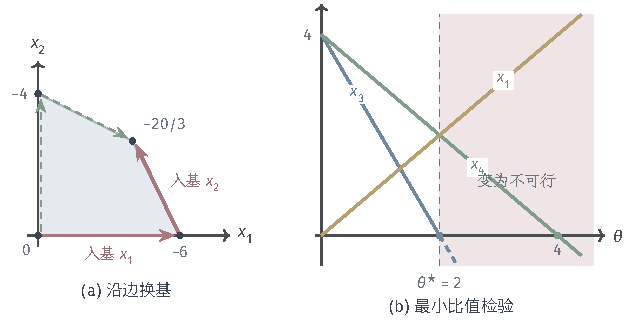
\includegraphics[width=107.262mm]{figures/03-optimization-evolution-and-signals/01-optimization/tikz/c2-simplex-path/figure.pdf}
  \caption{单纯形法沿边换基。(a) 红色实线箭头是表~\ref{tab:opt-lp-simplex-run}中的路径：$x_1$入基走到$(2,0)$，$x_2$入基走到$(4/3,4/3)$；顶点旁的数是标准型目标值$\bm c^\top\bm x$。绿色虚线是先让$x_2$入基的另一条路径。(b) 第$0$轮的最小比值检验：沿边移动步长$\theta$时，基变量$x_3=4-2\theta$与$x_4=4-\theta$线性减小，$x_3$在$\theta^\star=2$处先降到零；浅红区域内$x_3<0$，点已离开可行域。}
  \label{fig:opt-lp-simplex-path}
\end{figure}

\paragraph{与网络单纯形法对照}
图上的最小费用流问题也是标准型线性规划：每条弧$(i,j)$上的流量是一个变量，每个顶点一条守恒约束“净流出等于供需量”，所以弧$(i,j)$对应的列在第$i$行为$1$、第$j$行为$-1$，其余为零。网络单纯形法利用了这一特殊结构，把本节的每一步都换成图上的操作；其树基、节点势和沿环调整的完整推导，可参考\BookChapterRef{chap:graph-optimization}{卷一“图上的组合优化”章}。各行之和为零，所以这些行线性相关；对连通网络删去一行（相当于固定一个根顶点的势为零）后矩阵满行秩，此时基恰好对应生成树。表~\ref{tab:opt-lp-network-simplex}列出了逐项对应。网络单纯形法每一步都只沿树做加减，不需要一般的矩阵分解，这正是特殊结构带来的好处；但这一结构不能代替一般的单纯形法，后者处理的是任意矩阵$\bm A$。卷一的版本还直接处理弧的上界，入弧自身先到达上界时发生“界翻转”；本节只讨论$\bm x\ge\bm 0$的标准型，带上界的变量需要相应推广。

\begin{table}[!htbp]
  \centering
  \caption{一般单纯形法与网络单纯形法的对应。左列是本节的矩阵运算，右列是最小费用流中利用关联矩阵结构实现的同一操作。}
  \label{tab:opt-lp-network-simplex}
  \begin{tabular}{@{}ll@{}}
    \toprule
    一般单纯形法 & 网络单纯形法 \\
    \midrule
    约束行$\bm A\bm x=\bm b$ & 顶点的流量守恒 \\
    列$\bm a_j$ & 弧$(i,j)$，列为$\bm e_i-\bm e_j$ \\
    基$B$ & 生成树的树弧 \\
    乘子$\bm y=\bm A_B^{-\top}\bm c_B$ & 节点势$\bm\pi$（树弧约化费用为零） \\
    约化费用$c_j-\bm a_j^\top\bm y$ & $c_{i,j}-\pi_i+\pi_j$ \\
    方向$\bm d_B=-\bm A_B^{-1}\bm a_j$ & 沿基本环调整流量 \\
    最小比值检验 & 环上剩余量的最小值 \\
    出基变量 & 出弧（阻塞弧） \\
    \bottomrule
  \end{tabular}
\end{table}

\subsection{初始可行基与两阶段法}
\label{sec:opt-lp-two-phase}

算法~\ref{alg:opt-lp-simplex}要求从一个可行基出发。资源模型的约束都是“$\le$”且右端非负，松弛变量的列组成单位矩阵，原点就是基本可行解。这只是幸运的情形。若作坊还承诺两种产品每天合计至少生产$1$件，即$x_1+x_2\ge1$，减去剩余变量$x_5$后写成$x_1+x_2-x_5=1$；这时以$\{3,4,5\}$为基得到$x_5=-1<0$，原点不再可行，也没有现成的单位列可用。一般标准型更是如此，需要专门寻找起点。

\paragraph{第一阶段：构造一个容易起步的辅助问题}
先把$b_i<0$的行整行乘以$-1$，使$\bm b\ge\bm 0$；这不改变可行域。再为每一行引入一个\term{人工变量}（artificial variable）$a_i\ge0$，考虑辅助问题
\begin{equation}
\label{eq:opt-lp-phase-one}
  \min_{\bm x,\bm a}\ \bm 1^\top\bm a
  \quad\text{s.t.}\quad
  \bm A\bm x+\bm a=\bm b,\quad \bm x\ge\bm 0,\quad \bm a\ge\bm 0.
\end{equation}
人工变量的列组成单位矩阵，$(\bm x,\bm a)=(\bm 0,\bm b)$就是它的基本可行解，所以辅助问题有现成的起点；系数矩阵$[\bm A\ \bm I]$也总是满行秩。目标$\bm 1^\top\bm a$不小于零，有下界，配合下一小节的防循环规则，单纯形法会在有限步后停在辅助问题的一个最优基本可行解上。人工变量衡量的是原等式还差多少才能满足，第一阶段就是设法把这些差额压到零。在实际计算中，已有松弛变量可用的行不必再加人工变量，松弛变量的列可以直接充当单位列。

\begin{theorem}[第一阶段的判定]
\label{thm:opt-lp-phase-one}
原问题的可行域$P$非空，当且仅当辅助问题~\eqref{eq:opt-lp-phase-one}的最优值为零。最优值为零时，最优解中的$\bm x$属于$P$。
\end{theorem}

\begin{proof}
若$\bm x\in P$，则$(\bm x,\bm 0)$对辅助问题可行且目标为零，而目标不可能为负，所以最优值为零。反过来，最优值为零时最优解满足$\bm a=\bm 0$，于是$\bm A\bm x=\bm b$、$\bm x\ge\bm 0$。
\end{proof}

第一阶段因此有两种结局。最优值为正时，原问题不可行；第~\ref{sec:opt-lp-certificates}节将说明，此时的终止基还能给出一份可以独立核对的不可行证书。最优值为零时，得到了原问题的一个可行点，但还需要把它整理成原问题的可行基。

\paragraph{把人工变量移出基}
最优值为零时所有人工变量都等于零，但某些人工变量可能仍在基中，只是取值为零。不能直接删去这些列，否则剩下的列数少于行数，基矩阵不再是可逆方阵。设人工变量$a_k$在基中的位置对应$\bm A_B^{-1}$的第$r$行，记该行为$\bm w^\top$。对每个原变量$x_j$，$\bm w^\top\bm a_j$是用当前基表示$\bm a_j$时$a_k$所占的系数。分两种情况：
\begin{itemize}
  \item 若某个非基原变量$x_j$满足$\bm w^\top\bm a_j\ne0$，就让$x_j$入基、$a_k$出基。由引理~\ref{lem:opt-lp-pivot}的证明，新的基矩阵可逆；$a_k=0$，所以这是步长为零的换基，点不动，目标仍为零。
  \item 若全部原变量都满足$\bm w^\top\bm a_j=0$，即$\bm w^\top\bm A=\bm 0^\top$，而$\bm w\ne\bm 0$（它是可逆矩阵的一行），说明$\bm A$的行线性相关。取$w_i\ne0$的某一行$i$，它是其余行的线性组合；原系统可行，所以这一行对应的方程也由其余方程推出，可以删去。
\end{itemize}
重复处理，直到基中没有人工变量。剩下的基全部由原变量组成，是原问题（删去冗余行后）的可行基。随后恢复原目标$\bm c$，从这个基出发运行算法~\ref{alg:opt-lp-simplex}，称为第二阶段。两个阶段合起来就是\term{两阶段法}（two-phase method）。若事先已知$\bm A$满行秩，第二种情况不会出现。

\begin{example}[带最低产量的资源模型]
\label{ex:opt-lp-two-phase}
在资源模型中加入$x_1+x_2-x_5=1$，变量依次为$x_1,\dots,x_5$与人工变量$a$。前两行用松弛变量$x_3,x_4$，第三行用人工变量，初始基为$\{x_3,x_4,a\}$，基本可行解$x_3=x_4=4$、$a=1$。第一阶段目标只对$a$计费用$1$，乘子$\bm y=(0,0,1)^\top$，约化费用$\bar c_1=\bar c_2=-1$、$\bar c_5=1$。让$x_1$入基，$x_1$每增加一单位，$x_3,x_4,a$分别减少$2,1,1$，比值为$2,4,1$，所以$a$出基，步长为$1$。此时$\bm x=(1,0,2,3,0)^\top$，人工变量已经为零，第一阶段最优值为零，基$\{x_1,x_3,x_4\}$是原问题的可行基。

第二阶段恢复$\bm c=(-3,-2,0,0,0)^\top$。在基$\{x_1,x_3,x_4\}$下解得$\bm y=(0,0,-3)^\top$，$\bar c_2=1$、$\bar c_5=-3$，于是$x_5$入基、$x_3$出基，步长$1$，到达$(2,0)$；再让$x_2$入基、$x_4$出基，步长$4/3$，到达$(4/3,4/3)$，此时$x_5=5/3$，约化费用全部非负。整个过程依次经过$(0,0)$、$(1,0)$、$(2,0)$、$(4/3,4/3)$，其中第一个点只对辅助问题可行。
\end{example}

图~\ref{fig:opt-lp-two-phase-flow}汇总了两阶段法的流程。注意它的每一种结局都带有可以核对的数据：可行性由第一阶段判定，最优或无下界由第二阶段判定。

\begin{figure}[!htbp]
  \centering
  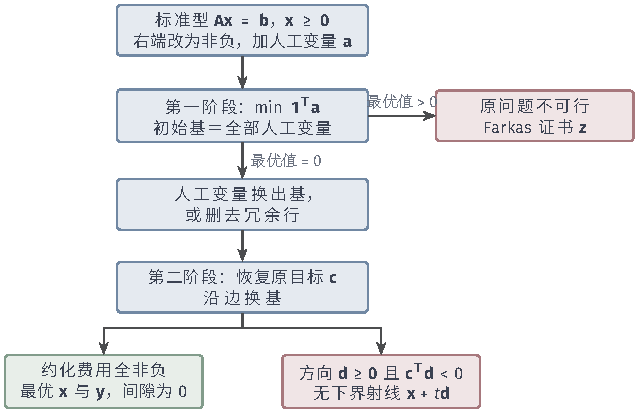
\includegraphics[width=108.112mm]{figures/03-optimization-evolution-and-signals/01-optimization/tikz/c2-two-phase-flow/figure.pdf}
  \caption{两阶段法的流程与三种结局。第一阶段从人工变量组成的单位基出发，最小化人工变量之和：最优值为正时原问题不可行，并得到Farkas证书（第~\ref{sec:opt-lp-certificates}节）；最优值为零时把人工变量换出基或删去冗余行，进入第二阶段。第二阶段以原目标换基，停止时或者得到约化费用全部非负的最优基，或者得到使目标无限下降的可行射线（红框为原问题没有有限最优解的两种情形）。}
  \label{fig:opt-lp-two-phase-flow}
\end{figure}

\subsection{退化、循环与有限终止}
\label{sec:opt-lp-degeneracy}

每次换基目标都不增，基又只有有限个，单纯形法是否一定会停？只有当每一步目标都严格下降时，才能断定不会回到已经访问过的基，从而有限终止。退化恰好破坏这一点。

\paragraph{零步长的换基}
回到第~\ref{sec:opt-lp-bases}小节加了市场限制$x_1\le2$的模型，变量为$x_1,\dots,x_5$，初始基$\{3,4,5\}$。$x_1$入基时，三个比值为$x_3{:}\,4/2=2$、$x_4{:}\,4/1=4$、$x_5{:}\,2/1=2$，$x_3$与$x_5$同时达到最小值。若让$x_5$出基，到达$(2,0)$，基为$\{1,3,4\}$，其中$x_3=0$。

下一轮$\bm y=(0,0,-3)^\top$，$\bar c_2=-2$，$x_2$入基。解$\bm A_B\bm u=\bm a_2$得$x_1,x_3,x_4$随$x_2$增加分别减少$0,1,2$；$x_3$的比值是$0/1=0$，所以$\theta^\star=0$。换基后基变为$\{1,2,4\}$，点仍是$(2,0)$，目标仍是$-6$：这就是一次\term{退化换基}（degenerate pivot）。再下一轮$\bar c_5=-1$，$x_5$入基、$x_4$出基，步长$2/3$，到达$(4/3,4/3)$。图~\ref{fig:opt-lp-degenerate-vertex}画出了这条路径：中间那一步换了基，却没有移动。这里的零步长并非白费，它把$x_2$换进了基，使下一步能沿正确的边离开；但它也说明“目标不增”本身不能保证进展。若在第一步的并列中改让$x_3$出基，则直接得到基$\{1,4,5\}$，下一步一次走到最优点。

\begin{figure}[!htbp]
  \centering
  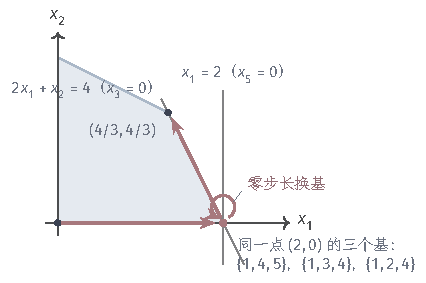
\includegraphics[width=72.164mm]{figures/03-optimization-evolution-and-signals/01-optimization/tikz/c2-degenerate-vertex/figure.pdf}
  \caption{退化顶点与零步长换基。加入$x_1\le2$后可行域不变，但顶点$(2,0)$上有三条边界同时取等号：$x_2=0$、$2x_1+x_2=4$与$x_1=2$。三个不同的基表示这一点。红色路径先从原点走到$(2,0)$，在原地做一次步长为零的换基（小圆弧），再走到最优点$(4/3,4/3)$。}
  \label{fig:opt-lp-degenerate-vertex}
\end{figure}

\paragraph{循环}
若零步长换基接连发生，算法可能在若干个表示同一点的基之间兜圈子，回到已经出现过的基，此后按同样的规则重复同一串换基而永不停止。把“基的序列中某个基重复出现”称为\term{循环}（cycling）。要区分两件事：多个基表示同一点只是退化，本身无害；算法回到同一个基才是循环。已知存在具体的线性规划，在最负约化费用入基、并列时任意选择出基的规则下发生循环\scite{math-bertsimas1997linear}。因此出入基的选择必须写进算法。

\paragraph{Bland规则}
最简单的防循环规则只看变量的编号，它由Bland提出\scite{math-bland1977finite}。

\begin{definition}[Bland规则]
\label{def:opt-lp-bland}
在算法~\ref{alg:opt-lp-simplex}中，入基时在全部$\bar c_j<0$的非基变量中选编号最小的；出基时在式~\eqref{eq:opt-lp-ratio-test}中达到最小比值的全部基变量中选编号最小的。这一选法称为\term{Bland规则}（Bland's rule）。
\end{definition}

\begin{theorem}[Bland规则不会循环]
\label{thm:opt-lp-bland}
设$\bm A$满行秩。按Bland规则执行算法~\ref{alg:opt-lp-simplex}，不会出现循环。
\end{theorem}

\begin{proof}
假设出现循环，基序列$B^{(0)},B^{(1)},\dots,B^{(k)}=B^{(0)}$。目标值沿途不增，又回到原值，所以每次换基的步长都是零，整个循环中基本可行解始终是同一点$\bm x$。称循环中至少有一次入基的变量为“变动变量”；它在某个基中是非基变量，所以$x_j=0$。记变动变量中编号最大的为$t$。

在循环中取一个$x_t$出基的基$B$，设此时入基的是$x_s$；$s$也是变动变量，故$s<t$。沿这次换基的方向$\bm d$（式~\eqref{eq:opt-lp-direction}）有$\bm A\bm d=\bm 0$、$d_s=1$、$\bm c^\top\bm d=\bar c_s<0$；$x_t$出基说明$d_t<0$。再取循环中一个$x_t$入基的基$B'$，记它的乘子为$\bm y'$、约化费用为$\bar{\bm c}'=\bm c-\bm A^\top\bm y'$。Bland规则选中$t$，说明$\bar c'_t<0$，而编号小于$t$的变量都有$\bar c'_j\ge0$；基变量的约化费用为零。

由$\bm A\bm d=\bm 0$，
\[
  \sum_{j=1}^n\bar c'_jd_j=\bm c^\top\bm d-\bm y'^\top\bm A\bm d=\bar c_s<0,
\]
所以存在$r$使$\bar c'_rd_r<0$。$d_r\ne0$说明$r\in B$或$r=s$；$\bar c'_r\ne0$说明$r\notin B'$。$r$在$B$或下一个基中是基变量，在$B'$中是非基变量，所以它是变动变量，$r\le t$。逐一排除：$r=t$时$\bar c'_t<0$且$d_t<0$，乘积为正；$r=s$时$s<t$，$\bar c'_s\ge0$而$d_s=1$，乘积非负。所以$r\in B$、$r<t$，于是$\bar c'_r\ge0$，结合乘积为负得$\bar c'_r>0$、$d_r<0$。但$r$是变动变量，$x_r=0$，在基$B$的比值检验中它的比值是$0/(-d_r)=0=\theta^\star$，与$x_t$并列达到最小值；Bland规则应当选编号更小的$r$出基，而不是$t$。矛盾。
\end{proof}

\begin{theorem}[单纯形法的有限终止]
\label{thm:opt-lp-finite}
设$\bm A$满行秩，从一个可行基出发按Bland规则执行算法~\ref{alg:opt-lp-simplex}（精确算术）。算法在有限轮后停止，要么得到满足$\bar{\bm c}_N\ge\bm 0$的最优基本可行解，要么得到满足$\bm A\bm d=\bm 0$、$\bm d\ge\bm 0$、$\bm c^\top\bm d<0$的方向，说明问题无下界。
\end{theorem}

\begin{proof}
基至多有$\binom nm$个。若算法永不停止，基序列中必有某个基重复出现，形成循环，与定理~\ref{thm:opt-lp-bland}矛盾。算法只在算法~\ref{alg:opt-lp-simplex}的两个返回处停止，两种结论分别由定理~\ref{thm:opt-lp-optimality-criterion}和最小比值检验前的讨论给出。
\end{proof}

两个定理分工明确：有限个基保证序列不能无限地“不重复”，防循环规则保证序列不会“重复”，二者合起来才推出有限终止。同一结论也适用于第一阶段的辅助问题，它的系数矩阵$[\bm A\ \bm I]$满行秩。

\paragraph{代价}
有限终止不等于快。每轮代价由两部分组成：解两个$m$阶线性方程组，以及对至多$n-m$个非基列计算约化费用，后者正比于$\bm A$的非零元个数。总代价还要乘以换基次数，而有限终止的论证只给出“不超过基的个数”这一上界。这个上界不是虚设的：Klee与Minty构造了一族$d$维的变形立方体，在最负约化费用规则下单纯形法要访问全部$2^d$个顶点\scite{math-klee1972simplex}。因此不能从有限终止推出多项式时间保证。在许多实际问题上单纯形法换基次数并不多，但这是经验观察，不是定理。与此对照，第~\ref{chap:constrained-optimization}章介绍的内点法有多项式时间的复杂度保证。此外，以上讨论都假设精确算术；输入数据的位数和舍入误差会影响实际计算，下一小节讨论这一点。

\subsection{单纯形法的数值实现}
\label{sec:opt-lp-revised-simplex}

公式中的$\bm A_B^{-1}$便于推导，却不宜照字面计算。显式求逆每轮要$O(m^3)$次运算，舍入误差也比解方程组更大。

\paragraph{两个线性方程组}
算法~\ref{alg:opt-lp-simplex}只需要逆矩阵与向量的乘积，可以改写为两个方程组：
\[
  \bm A_B^\top\bm y=\bm c_B,\qquad
  \bm A_B\bm u=\bm a_j.
\]
前者给出乘子与约化费用，后者给出方向$\bm d_B=-\bm u$；两者共用同一个基矩阵。保存$\bm A_B$的一个LU分解，两个方程组就都只需前代与回代。只维护基矩阵的分解、而不维护整张表格的实现，称为\term{修正单纯形法}（revised simplex method）\scite{math-nocedal2006numerical}。

\paragraph{更新与重新分解}
相邻两个基只差一列，基矩阵的变化是一个秩一修正，分解可以借助低秩更新而不必重算。但更新会累积舍入误差，大型稀疏问题中还会使分解因子逐渐变稠，所以实现中每隔若干轮（或在误差指标变差时）重新分解一次。$\bm A$通常很稀疏，选择分解的主元次序时要兼顾数值稳定和保持稀疏；定价也不必每轮扫描全部列，可以只检查一部分候选列。这些都改变每轮的实际代价，但不改变算法的数学步骤。

\paragraph{在原模型上检验}
浮点计算得到的$\bm x$不会精确满足等式。设算法报告了基$B$与解$\bm x$，应回到原模型逐项检查：等式残差$\lVert\bm A\bm x-\bm b\rVert$，变量的负部$\max_j\max\{-x_j,0\}$，重新计算的目标值，以及约化费用$\bar c_j$的符号。例如把资源模型的最优解存成七位小数$\bm x=(1.333\,333\,3,\ 1.333\,333\,3,\ 0,\ 0)^\top$，等式残差约为$10^{-7}$，它只是近似可行。容差应当按数据的尺度设置，例如与$\lVert\bm A\rVert$、$\lVert\bm b\rVert$、$\lVert\bm c\rVert$成比例，而不是取一个绝对的小数。

两类情形需要特别留意。约化费用接近零时，它的符号可能由舍入误差决定，算法可能把本应停止的状态当作可以改进，或者反过来；基矩阵接近奇异时，解出的$\bm x_B$和$\bm y$对扰动很敏感，残差小也不代表解准确。因此要分清三件事：算法按规则停止了，结果的残差很小，以及结果已经被证明是原问题的最优解。前两件事都不蕴含第三件。精确算术中，定理~\ref{thm:opt-lp-optimality-criterion}给出了证明；有限精度下，需要一个不依赖算法过程、能直接核对的界，下一节的对偶问题提供的正是这样的界。

\section{对偶问题与解的证书}
\label{sec:opt-lp-duality}

单纯形法报告“$(4/3,4/3)$最优，获利$20/3$”。别人若不想重跑算法，怎样确认这句话？验证可行性很容易，代入约束即可；难的是确认没有更好的产量。本节从“给获利找一个上界”出发，把约束按非负权重相加，得到线性规划的对偶问题。原问题和对偶问题互相给出界，二者同值时就证明了最优；单纯形法停止时的乘子$\bm y$恰好就是这样一组权重。同样的思路还为“不可行”和“无下界”分别给出可以核对的证据。

\subsection{对偶的构造与弱对偶}
\label{sec:opt-lp-weak-duality}

\paragraph{把约束加起来}
在资源模型~\eqref{eq:opt-lp-resource}中，把第一条原料约束乘以$u_1\ge0$，第二条乘以$u_2\ge0$，相加得
\[
  (2u_1+u_2)x_1+(u_1+2u_2)x_2\le4u_1+4u_2.
\]
若权重满足$2u_1+u_2\ge3$与$u_1+2u_2\ge2$，则由$x_1,x_2\ge0$，左边不小于获利$3x_1+2x_2$，于是任何可行产量的获利都不超过$4u_1+4u_2$。例如$\bm u=(1,1)$给出上界$8$，$\bm u=(2,1)$给出上界$10$，$\bm u=(4/3,1/3)$给出上界$20/3$。最后一个上界恰好等于$(4/3,4/3)$的获利，所以不可能有更好的产量。这一行推导不依赖任何算法，任何人都能复核。

权重可以解释为原料的价格。设想有人想把作坊的全部原料买下，给两种原料分别出价$u_1,u_2$。作坊只有在“把做一件产品所需的原料卖掉”至少不比“做成产品卖掉”少赚时才愿意出售，即$2u_1+u_2\ge3$、$u_1+2u_2\ge2$；买方则希望总价$4u_1+4u_2$尽量低。买方的问题
\begin{equation}
\label{eq:opt-lp-resource-dual}
  \min_{u_1,u_2}\ 4u_1+4u_2
  \quad\text{s.t.}\quad
  2u_1+u_2\ge3,\quad u_1+2u_2\ge2,\quad u_1,u_2\ge0
\end{equation}
就是在寻找最紧的上界。图~\ref{fig:opt-lp-dual-bounds}(a)画出了价格的可行域，它在$(4/3,1/3)$处取得最小总价$20/3$。

\begin{figure*}[!htbp]
  \centering
  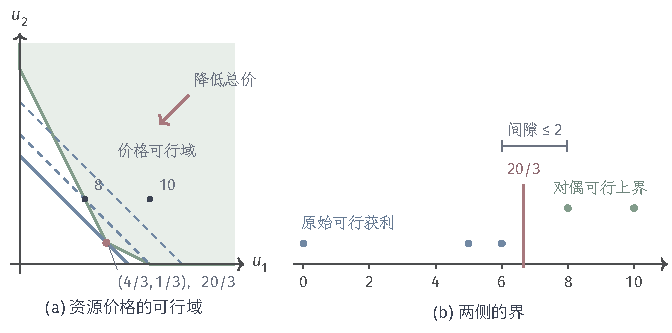
\includegraphics[width=113.771mm]{figures/03-optimization-evolution-and-signals/01-optimization/tikz/c2-dual-bounds/figure.pdf}
  \caption{原料价格给出的上界。(a) 绿色区域是满足式~\eqref{eq:opt-lp-resource-dual}约束的价格$(u_1,u_2)$，蓝色线是总价$4u_1+4u_2$的等值线，实线为最小总价$20/3$，在红点$(4/3,1/3)$处取得；黑点$(1,1)$与$(2,1)$也可行，总价为$8$和$10$。(b) 数轴上，蓝点是可行产量$(0,0)$、$(1,1)$、$(2,0)$的获利$0,5,6$，绿点是可行价格的总价$8,10$。每个蓝点都在每个绿点左侧；最优获利与最小总价都在$20/3$处，由$6$与$8$已能确定最优值落在长度为$2$的区间内。}
  \label{fig:opt-lp-dual-bounds}
\end{figure*}

\paragraph{标准型的对偶问题}
对标准型~\eqref{eq:opt-lp-standard}做同样的事。约束是等式，任意符号的权重都不改变等号方向，所以给第$i$个等式配一个可正可负的权重$y_i$。若$\bm A^\top\bm y\le\bm c$，则对任意可行$\bm x$，
\[
  \bm b^\top\bm y=(\bm A\bm x)^\top\bm y=\bm x^\top(\bm A^\top\bm y)\le\bm x^\top\bm c,
\]
不等号用到了$\bm x\ge\bm 0$：对非负的$x_j$，把系数$(\bm A^\top\bm y)_j$放大为$c_j$只会使乘积变大。于是每个满足$\bm A^\top\bm y\le\bm c$的$\bm y$都给出原问题最优值的一个下界$\bm b^\top\bm y$，最好的下界由下面的问题给出。

\begin{definition}[线性规划的对偶问题]
\label{def:opt-lp-dual}
标准型~\eqref{eq:opt-lp-standard}的\term{对偶问题}（dual problem）是
\begin{equation}
\label{eq:opt-lp-dual}
  \max_{\bm y\in\mathbb R^m}\ \bm b^\top\bm y
  \quad\text{s.t.}\quad
  \bm A^\top\bm y\le\bm c.
\end{equation}
相对地，称式~\eqref{eq:opt-lp-standard}为\term{原始问题}（primal problem）。满足对偶约束的$\bm y$称为对偶可行。
\end{definition}

\begin{theorem}[弱对偶]
\label{thm:opt-lp-weak-duality}
若$\bm x$对原始问题可行、$\bm y$对对偶问题可行，则$\bm b^\top\bm y\le\bm c^\top\bm x$。特别地，若二者相等，则$\bm x$与$\bm y$分别是两个问题的最优解。
\end{theorem}

上面的推导就是证明。第二句成立是因为：任何其他原始可行点的目标值都不小于$\bm b^\top\bm y=\bm c^\top\bm x$，任何其他对偶可行点的目标值都不大于$\bm c^\top\bm x=\bm b^\top\bm y$。这就是\term{弱对偶}（weak duality）。差$\bm c^\top\bm x-\bm b^\top\bm y\ge0$称为这对可行点的\term{对偶间隙}（duality gap），它同时控制了两侧离最优值有多远：$\bm c^\top\bm x-f^\star\le\bm c^\top\bm x-\bm b^\top\bm y$。间隙为零就证明了最优，而且只需要核对两组可行性和两个数是否相等，不需要第~\ref{chap:constrained-optimization}章的一般KKT理论。

\paragraph{符号规则来自同一个推导}
不同形式的原始约束对应不同的对偶符号，但不必死记表格：每次都回到“加权相加后仍保持不等号方向”这一推导即可。以资源模型为例，它是最大化问题，约束取“$\le$”，可行的获利是最优值的下界；要得到上界，“$\le$”约束的权重必须非负，否则乘以负数会把不等号反向，这就是$u_1,u_2\ge0$的来历；变量非负，所以只需权重组合后的系数“盖住”获利系数，得到$\ge$型的对偶约束。把资源模型写成例~\ref{ex:opt-lp-resource-standard}的标准型再套用式~\eqref{eq:opt-lp-dual}，对偶约束为$2y_1+y_2\le-3$、$y_1+2y_2\le-2$、$y_1\le0$、$y_2\le0$（后两条来自松弛变量的列），令$\bm u=-\bm y$即得式~\eqref{eq:opt-lp-resource-dual}，两种写法一致。最小化问题中原始值在上、对偶值在下；最大化问题中方向相反。图~\ref{fig:opt-lp-dual-bounds}(b)把最大化例子中两侧的界画在同一条数轴上。

\subsection{强对偶与互补松弛}
\label{sec:opt-lp-strong-duality}

弱对偶只说明下界不超过上界。我们关心的是：最好的下界是否恰好等于最优值？对线性规划，单纯形法的终止状态直接给出肯定的回答。

\begin{theorem}[线性规划强对偶]
\label{thm:opt-lp-strong-duality}
若标准型~\eqref{eq:opt-lp-standard}可行且目标在可行域上有下界，则原始问题与对偶问题~\eqref{eq:opt-lp-dual}都有最优解，并且两个最优值相等。
\end{theorem}

\begin{proof}
先把$\bm A$化为满行秩。原问题可行，等式系统相容；删去冗余行后得到$\bm A'\bm x=\bm b'$，可行域不变。若$\bm y'$对删行后的问题对偶可行，把删去的行对应的分量补为零得到$\bm y$，则$\bm A^\top\bm y=\bm A'^\top\bm y'$、$\bm b^\top\bm y=\bm b'^\top\bm y'$，所以对偶可行性和对偶目标值都不变。下面设$\bm A$满行秩。

对原问题执行两阶段法，两个阶段都使用Bland规则。由定理~\ref{thm:opt-lp-phase-one}与定理~\ref{thm:opt-lp-finite}，第一阶段在有限步后停止，最优值为零（原问题可行），把人工变量换出基后得到可行基。第二阶段同样在有限步后停止；由于目标有下界，不会以无下界方向结束，所以停在满足$\bar{\bm c}_N\ge\bm 0$的基$B$上，基本可行解记为$\bm x^\star$。

令$\bm y^\star=\bm A_B^{-\top}\bm c_B$。约化费用$\bar{\bm c}=\bm c-\bm A^\top\bm y^\star$在基指标上为零，在非基指标上非负，所以$\bm A^\top\bm y^\star\le\bm c$，$\bm y^\star$对偶可行。又
\[
  \bm b^\top\bm y^\star=\bm b^\top\bm A_B^{-\top}\bm c_B=\bm c_B^\top\bm A_B^{-1}\bm b=\bm c_B^\top\bm x^\star_B=\bm c^\top\bm x^\star.
\]
由弱对偶，$\bm x^\star$与$\bm y^\star$分别最优，且最优值相等。
\end{proof}

原始与对偶最优值相等的结论称为\term{强对偶}（strong duality）。证明说明了单纯形法中乘子$\bm y$的身份：它就是对偶最优解，而“约化费用全部非负”与“$\bm y$对偶可行”是同一件事。在资源模型中，表~\ref{tab:opt-lp-simplex-run}最后一轮的$\bm y=(-4/3,-1/3)^\top$，对应价格$\bm u=-\bm y=(4/3,1/3)$，正是图~\ref{fig:opt-lp-dual-bounds}(a)的最优价格。这一强对偶结论只要求原问题可行、有下界，不需要任何内点条件；第~\ref{chap:constrained-optimization}章讨论一般凸问题时，零间隙要借助Slater条件之类的额外假设，那是线性结构以外才需要的。

\paragraph{互补松弛}
对一对可行点，把间隙展开：
\[
  \bm c^\top\bm x-\bm b^\top\bm y=\bm c^\top\bm x-(\bm A\bm x)^\top\bm y=\bm x^\top(\bm c-\bm A^\top\bm y)=\sum_{j=1}^nx_j\,(c_j-\bm a_j^\top\bm y).
\]
求和中的每一项都是两个非负数的乘积，所以间隙为零当且仅当每一项都为零。

\begin{theorem}[互补松弛]
\label{thm:opt-lp-complementary-slackness}
设$\bm x$原始可行、$\bm y$对偶可行。二者同为最优解，当且仅当对每个$j$，
\[
  x_j\,(c_j-\bm a_j^\top\bm y)=0,
\]
即$x_j>0$时第$j$条对偶约束取等号，第$j$条对偶约束严格成立时$x_j=0$。
\end{theorem}

\begin{proof}
若二者都最优，由定理~\ref{thm:opt-lp-strong-duality}，两侧最优值相等（原问题有可行点，又有对偶可行点给出下界），间隙为零，各项均为零。反之各项为零时间隙为零，由弱对偶二者最优。
\end{proof}

这一条件称为\term{互补松弛}（complementary slackness）。在资源模型中，$\bm x^\star=(4/3,4/3,0,0)^\top$，$\bm c-\bm A^\top\bm y^\star=(0,0,4/3,1/3)^\top$，逐项乘积全为零，两侧值都是$-20/3$（最大化写法中都是$20/3$）。翻译回资源语言：两种产品都在生产（$x_1,x_2>0$），所以每件产品的获利恰好等于它消耗的原料按价格折算的价值，$2\cdot\frac43+\frac13=3$、$\frac43+2\cdot\frac13=2$；两种原料都有正价格，所以它们都被用完（松弛变量$x_3=x_4=0$）。反过来，有剩余的原料价格必为零：多出来的原料不值钱。

\paragraph{最优面是一个面}
互补松弛还说明了第~\ref{sec:opt-lp-polyhedra}节中“最优面”这一名称的来由。取定一个对偶最优解$\bm y^\star$，可行点$\bm x$最优当且仅当$x_j=0$对每个满足$c_j-\bm a_j^\top\bm y^\star>0$的$j$成立。所以标准型的全部最优解恰好是让这些非负约束同时取等号所得的面。在图~\ref{fig:opt-lp-optimal-face}(b)中，最优价格只让第一种原料的松弛变量必须为零，最优面就是$x_3=0$那条边。

\paragraph{有限精度下怎样报告}
数值求解器给出的$\bm x$与$\bm y$通常各自只近似可行。此时应同时报告四个量：原始等式残差$\lVert\bm A\bm x-\bm b\rVert$、原始变量的负部、对偶约束的违反量$\max_j\max\{\bm a_j^\top\bm y-c_j,0\}$，以及间隙$\bm c^\top\bm x-\bm b^\top\bm y$。只有在$\bm y$确实对偶可行时，$\bm b^\top\bm y$才是合法的下界；只有在$\bm x$确实可行时，$\bm c^\top\bm x$才是可以达到的值。不满足可行性的两个数之差不能直接当作误差上界。例如资源模型中取价格$\bm u=(1.4,0.2)$，它满足$2u_1+u_2\ge3$，却违反$u_1+2u_2\ge2$（左边为$1.8$）；它给出的“上界”$4u_1+4u_2=6.4$小于真实最优值$20/3$。若忽略这一点违反，就会错误地断言获利不可能超过$6.4$。

\subsection{不可行与无下界的证书}
\label{sec:opt-lp-certificates}

线性规划只有三种结局：有最优解、不可行、可行但无下界。前一小节为第一种结局给出了证书：一对原始、对偶可行点，间隙为零。另外两种结局也有类似的、可以独立核对的证据。

\paragraph{不可行的证书}
若再要求两种产品合计至少生产$5$件，资源模型就不可行。证据是什么？把两条原料约束各乘$1/3$相加，得到$x_1+x_2\le8/3$，与$x_1+x_2\ge5$矛盾。一般地，不可行性可以由一组权重这样“组合出矛盾”来证明，而且只要不可行，这样的权重一定存在。

\begin{theorem}[Farkas择一定理]
\label{thm:opt-lp-farkas}
给定$\bm A\in\mathbb R^{m\times n}$与$\bm b\in\mathbb R^m$，下面两个系统恰有一个有解：
\[
  \text{（甲）}\ \bm A\bm x=\bm b,\ \bm x\ge\bm 0;
  \qquad
  \text{（乙）}\ \bm A^\top\bm z\ge\bm 0,\ \bm b^\top\bm z<0.
\]
\end{theorem}

\begin{proof}
二者不能同时有解：否则$0>\bm b^\top\bm z=\bm x^\top\bm A^\top\bm z\ge0$，矛盾。

再设（甲）无解，构造（乙）的解。先把$b_i<0$的行乘以$-1$：记$\bm D$为对角元是$\pm1$的对角矩阵，使$\widetilde{\bm A}=\bm D\bm A$、$\widetilde{\bm b}=\bm D\bm b\ge\bm 0$。对$\widetilde{\bm A},\widetilde{\bm b}$构造第一阶段问题~\eqref{eq:opt-lp-phase-one}，按Bland规则求解。由定理~\ref{thm:opt-lp-finite}，它在有限步后停在一个最优基上，乘子记为$\bm w$，约化费用全部非负。原变量$x_j$的费用为$0$，所以$0-\widetilde{\bm a}_j^\top\bm w\ge0$，即$\widetilde{\bm A}^\top\bm w\le\bm 0$。最优值等于$\widetilde{\bm b}^\top\bm w$（与强对偶证明中的计算相同），由定理~\ref{thm:opt-lp-phase-one}和（甲）无解，它严格为正。令$\bm z=-\bm D\bm w$，则
\[
  \bm A^\top\bm z=-\bm A^\top\bm D\bm w=-\widetilde{\bm A}^\top\bm w\ge\bm 0,\qquad
  \bm b^\top\bm z=-\widetilde{\bm b}^\top\bm w<0.
\]
\end{proof}

满足（乙）的$\bm z$称为（甲）的不可行证书，这一结论通常称为\term{Farkas引理}（Farkas lemma）。核对它只需一次矩阵乘法：若有可行$\bm x$，则$\bm z^\top\bm b=\bm z^\top\bm A\bm x$是非负数$(\bm A^\top\bm z)_j$与非负数$x_j$乘积之和，不可能为负。证明的后半部分不是抽象的存在性论证：它说明第一阶段停止时的乘子$\bm w$取负号就是证书，求解器判定不可行时可以把它一并输出。

\begin{example}[合计至少五件]
\label{ex:opt-lp-farkas}
标准型变量为$x_1,\dots,x_5$，约束为$2x_1+x_2+x_3=4$、$x_1+2x_2+x_4=4$、$x_1+x_2-x_5=5$。第一阶段只需为第三行加人工变量。依Bland规则，$x_1$入基、$x_3$出基，再$x_2$入基、$x_4$出基，停在基$\{x_1,x_2,a\}$上，此时$x_1=x_2=4/3$，人工变量$a=7/3$，最优值$7/3>0$，乘子$\bm w=(-1/3,-1/3,1)^\top$。取$\bm z=-\bm w=(1/3,1/3,-1)^\top$，逐列核对$\bm A^\top\bm z$：$x_1$列$\tfrac23+\tfrac13-1=0$，$x_2$列$\tfrac13+\tfrac23-1=0$，$x_3,x_4,x_5$列分别为$\tfrac13,\tfrac13,1$，全部非负；而$\bm b^\top\bm z=\tfrac43+\tfrac43-5=-\tfrac73<0$。这组权重正是开头那句推理：两条原料约束各取$1/3$，再与产量要求相减。
\end{example}

图~\ref{fig:opt-lp-farkas}给出了定理的几何含义。$\{\bm A\bm x:\bm x\ge\bm 0\}$是$\bm A$的各列张成的锥$K$，（甲）有解就是$\bm b\in K$。当$\bm b$在锥外时，存在一个过原点的超平面$\{\bm v:\bm z^\top\bm v=0\}$，把整个锥留在$\bm z^\top\bm v\ge0$一侧，把$\bm b$放在另一侧；（乙）的两个条件说的正是这件事。

\begin{figure}[!htbp]
  \centering
  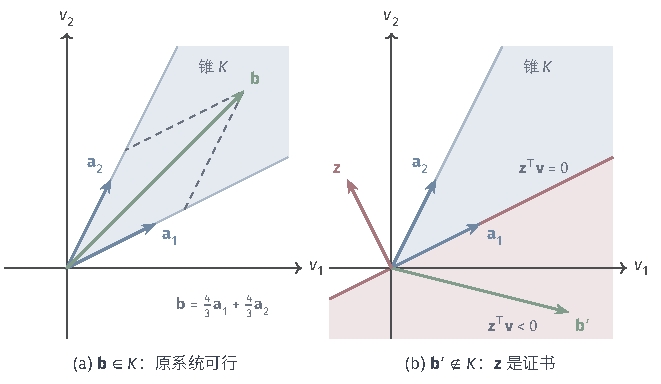
\includegraphics[width=111.898mm]{figures/03-optimization-evolution-and-signals/01-optimization/tikz/c2-farkas/figure.pdf}
  \caption{Farkas择一定理的几何。两列$\bm a_1=(2,1)$、$\bm a_2=(1,2)$张成锥$K$（浅蓝）。(a) $\bm b=(4,4)=\tfrac43\bm a_1+\tfrac43\bm a_2$在锥内，系统$\bm A\bm x=\bm b$、$\bm x\ge\bm 0$有解。(b) $\bm b'=(4,-1)$在锥外；$\bm z=(-1,2)$满足$\bm a_1^\top\bm z=0$、$\bm a_2^\top\bm z=3$、$\bm b'^\top\bm z=-6$，红线$\bm z^\top\bm v=0$把锥与$\bm b'$分在两侧，浅红半平面是$\bm z^\top\bm v<0$的一侧。}
  \label{fig:opt-lp-farkas}
\end{figure}

\paragraph{无下界的证书}
若原问题可行但无下界，证据是一个已知的可行点$\bm x_0$加一个方向$\bm d$，满足
\[
  \bm A\bm d=\bm 0,\qquad\bm d\ge\bm 0,\qquad\bm c^\top\bm d<0.
\]
核对很直接：对任意$t\ge0$，$\bm x_0+t\bm d$可行，目标$\bm c^\top\bm x_0+t\bm c^\top\bm d\to-\infty$。单纯形法在比值检验中发现$\bm d_B\ge\bm 0$时，返回的正是这样一对$(\bm x,\bm d)$。图~\ref{fig:opt-lp-polyhedron-cases}(c)是一个例子：标准型为$\min\ x_2-x_1$，约束$x_1+x_2-x_3=1$，$\bm x\ge\bm 0$；取$\bm x_0=(1,0,0)^\top$、$\bm d=(1,0,1)^\top$，有$\bm A\bm d=1+0-1=0$，$\bm c^\top\bm d=-1<0$。

\paragraph{三种不可行要分开}
原问题不可行、原问题无下界与对偶问题不可行是三件不同的事，它们之间只有部分蕴含关系。由弱对偶，原问题无下界时不可能有对偶可行点，否则它会给出有限下界，所以对偶问题不可行；上面的例子中对偶约束为$y\le-1$、$y\le1$、$-y\le0$，确实无解。反方向需要额外条件：只有在已经知道原问题可行时，才能由对偶不可行推出原问题无下界，因为若原问题可行且有下界，定理~\ref{thm:opt-lp-strong-duality}会给出对偶最优解。若不知道原问题是否可行，这一推理不成立。例如
\[
  \min\ -x_1-x_2\quad\text{s.t.}\quad x_1-x_2=1,\quad -x_1+x_2=1,\quad\bm x\ge\bm 0
\]
的两个等式相加得$0=2$，原问题不可行；它的对偶约束$y_1-y_2\le-1$与$-y_1+y_2\le-1$相加得$0\le-2$，对偶问题也不可行。方向$\bm d=(1,1)^\top$满足$\bm A\bm d=\bm 0$、$\bm d\ge\bm 0$、$\bm c^\top\bm d=-2<0$，可是没有可行的起点，它不能说明任何东西“无下界”。所以报告无下界时，必须同时给出可行点和方向，二者缺一不可。

\section{参数敏感性}
\label{sec:opt-lp-sensitivity}

模型中的数据往往只是估计：明天的原料可能多到一些，产品价格可能变动。重新求解当然可以，但我们更想知道，已经求得的最优基在多大范围内仍然有效，最优值又以什么速率变化。本节固定约束矩阵$\bm A$，分别改变右端$\bm b$和目标系数$\bm c$。之所以把$\bm A$固定，是因为改变资源数量与改变单位产品的资源消耗是两种不同的扰动：前者只移动约束边界，后者改变边界的方向，会同时影响可行性和比较，需要另作分析。

两种改变的检查方法都来自同一个观察：基$B$保持最优，当且仅当它同时满足两组条件，即基本解可行（$\bm A_B^{-1}\bm b\ge\bm 0$）与约化费用非负（$\bm c_N-\bm A_N^\top\bm A_B^{-\top}\bm c_B\ge\bm 0$）。前一组只涉及$\bm b$，后一组只涉及$\bm c$。所以改变$\bm b$只需重新检查可行性，改变$\bm c$只需重新检查约化费用。

\subsection{约束右端的变化}
\label{sec:opt-lp-rhs}

\paragraph{原基保持最优的范围}
把右端改为$\bm b+\Delta\bm b$，保留原最优基$B$。约化费用只依赖$\bm A$与$\bm c$，没有变化，对偶解$\bm y=\bm A_B^{-\top}\bm c_B$也仍然对偶可行。变化的只是基本解：
\[
  \bm x_B(\Delta\bm b)=\bm A_B^{-1}(\bm b+\Delta\bm b).
\]
只要它非负，$B$就仍是可行基，而约化费用非负，于是$B$仍然最优。这组线性不等式就是$\Delta\bm b$的允许范围。

在资源模型中，原最优基$B=\{1,2\}$，$\bm A_B^{-1}=\tfrac13\bigl(\begin{smallmatrix}2&-1\\-1&2\end{smallmatrix}\bigr)$。只改变第一种原料，$b_1=4+\delta$，得
\[
  x_1=\frac{2(4+\delta)-4}{3}=\frac{4+2\delta}{3},\qquad
  x_2=\frac{-(4+\delta)+8}{3}=\frac{4-\delta}{3},
\]
二者非负当且仅当$-2\le\delta\le4$，即$b_1\in[2,8]$。在这个范围内，最优产量沿直线$x_1+2x_2=4$移动：第一种原料越多，越多地生产更耗它的第一种产品。图~\ref{fig:opt-lp-rhs-sensitivity}(a)画出了这一移动，$b_1=2$时最优点到达$(0,2)$，$b_1=8$时到达$(4,0)$。

\paragraph{影子价格}
在允许范围内，最优值为
\[
  \bm c_B^\top\bm A_B^{-1}(\bm b+\Delta\bm b)=\bm y^\top\bm b+\bm y^\top\Delta\bm b,
\]
增量是$\bm y^\top\Delta\bm b$。对偶变量于是有了直接的含义：$y_i$是第$i$个右端每增加一个单位时最优值的变化率。在资源模型的最大化写法中，最优获利为$\tfrac{20}3+\tfrac43\delta$：第一种原料每多一个单位，获利多$4/3$，这正是对偶解给它的价格$u_1=4/3$；同理第二种原料每单位值$u_2=1/3$，其允许范围也是$b_2\in[2,8]$。因此对偶最优解又称\term{影子价格}（shadow price）：它告诉作坊，在当前范围内，为多买一单位原料最多值得付多少钱。第二种原料的影子价格只有$1/3$，若市价高于此，就不值得为它扩产。

\paragraph{超出范围之后}
影子价格只在允许范围内有效。图~\ref{fig:opt-lp-rhs-sensitivity}(b)画出了最优获利$v(b_1)$在整个范围内的变化：
\[
  v(b_1)=\begin{cases}
    2b_1, & 0\le b_1\le2,\\[2pt]
    \tfrac{4b_1+4}{3}, & 2\le b_1\le8,\\[2pt]
    12, & b_1\ge8.
  \end{cases}
\]
$b_1<2$时原基给出$x_1<0$，需要换基，最优点变为$(0,b_1)$，此时只生产第二种产品，第一种原料是唯一的瓶颈，它的价格升到$2$；$b_1>8$时原基给出$x_2<0$，最优点停在$(4,0)$，第一种原料已经过剩，价格降为$0$。$b_1<0$时问题不可行。函数在$b_1=2$与$b_1=8$处有折点，各段斜率正是相应最优基的影子价格。在折点上，最优对偶解不唯一：例如$b_1=2$时，价格$(2,0)$与$(4/3,1/3)$给出的总价都是$4$，它们分别是左、右两侧的斜率。这时只说“影子价格是多少”已经不准确，左右的变化率并不相同。

\begin{figure*}[!htbp]
  \centering
  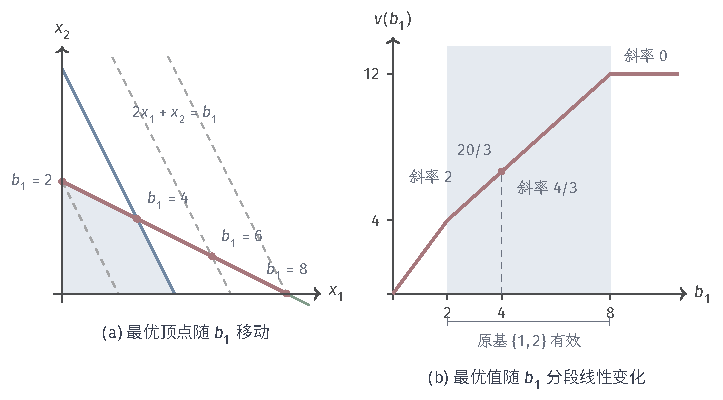
\includegraphics[width=122.357mm]{figures/03-optimization-evolution-and-signals/01-optimization/tikz/c2-rhs-sensitivity/figure.pdf}
  \caption{改变第一种原料的数量$b_1$（第二种固定为$4$）。(a) 蓝线是$b_1=4$时的边界$2x_1+x_2=4$，灰色虚线是$b_1=2,6,8$时的边界；红点是相应的最优顶点$((2b_1-4)/3,(8-b_1)/3)$，它们沿红线$x_1+2x_2=4$从$(0,2)$移到$(4,0)$。(b) 最优获利$v(b_1)$分三段线性变化，斜率依次为$2$、$4/3$、$0$；浅蓝区域$b_1\in[2,8]$内原基保持最优，斜率$4/3$就是第一种原料的影子价格，红点为$b_1=4$时的值$20/3$。}
  \label{fig:opt-lp-rhs-sensitivity}
\end{figure*}

这条折线是凹的，这不是巧合。若右端为$\bm b$与$\bm b'$时的最优解分别是$\bm x$与$\bm x'$，则对$\lambda\in[0,1]$，$\lambda\bm x+(1-\lambda)\bm x'$满足右端为$\lambda\bm b+(1-\lambda)\bm b'$的约束，所以最大化问题的最优值满足$v(\lambda\bm b+(1-\lambda)\bm b')\ge\lambda v(\bm b)+(1-\lambda)v(\bm b')$。凹性说明影子价格随资源增多而不增：资源越充裕，再多一单位的价值越低。对任意大的变化，影子价格仍然给出一个可靠的单侧界：设$\bm u$是右端为$\bm b$时的最优价格，它的可行性与右端无关，由弱对偶，对任何使问题可行的$\bm b'$都有$v(\bm b')\le\bm u^\top\bm b'=v(\bm b)+\bm u^\top(\bm b'-\bm b)$。所以“当前价格乘以变化量”在最大化问题中只是增量的上界，越出允许范围后可能严重高估，不能当作精确的预测。

\subsection{目标系数的变化}
\label{sec:opt-lp-cost}

\paragraph{原基保持最优的范围}
现在固定$\bm A$与$\bm b$，把目标系数改为$\bm c+\Delta\bm c$。原基本解$\bm A_B^{-1}\bm b$与$\bm c$无关，仍然可行；需要重新检查的是约化费用
\[
  \bar{\bm c}_N(\Delta\bm c)=(\bm c_N+\Delta\bm c_N)-\bm A_N^\top\bm A_B^{-\top}(\bm c_B+\Delta\bm c_B)\ge\bm 0.
\]
这一次保持不变的是可行点，重新变化的是候选之间的比较。

在资源模型中把第一种产品的获利改为$c_1$，最大化$c_1x_1+2x_2$。标准型中$\bm c_B=(-c_1,-2)^\top$，解$\bm A_B^\top\bm y=\bm c_B$得
\[
  y_1=\frac{2-2c_1}{3},\qquad y_2=\frac{c_1-4}{3},
\]
于是两个松弛变量的约化费用为$\bar c_3=-y_1=\tfrac{2c_1-2}3$、$\bar c_4=-y_2=\tfrac{4-c_1}3$。二者非负当且仅当$1\le c_1\le4$。在这个范围内顶点$(4/3,4/3)$保持最优，$c_1=3$时回到原来的数值$\bar c_3=4/3$、$\bar c_4=1/3$。

\paragraph{最优性锥}
这个范围有一个直观的几何解释。在顶点$(4/3,4/3)$处活跃的两条约束的外法向量是$(2,1)$与$(1,2)$。上面算出的$-\bm y$满足
\[
  (c_1,2)=\frac{2c_1-2}{3}(2,1)+\frac{4-c_1}{3}(1,2),
\]
即目标方向被写成两个法向量的组合，组合系数正是两种原料的价格。系数都非负，等价于目标方向落在两个法向量张成的锥中。图~\ref{fig:opt-lp-cost-sensitivity}(a)画出了这个锥：$c_1=3$的方向$(3,2)$在锥内，顶点最优；$c_1=6$的方向$(6,2)$转出了锥，沿边走向$(2,0)$会更好。$c_1=4$时方向$(4,2)$落在锥的边界上，与边$2x_1+x_2=4$垂直，$\bar c_4=0$，整条边都最优，这正是图~\ref{fig:opt-lp-optimal-face}(b)的情形（目标乘以正数不改变最优解）。$c_1=1$时方向$(1,2)$落在另一条边界上，最优面是通往$(0,2)$的边。

\paragraph{最优值的变化}
在原基保持最优的范围内，最优解不变，最优值随系数线性变化，变化率就是相应变量的取值：最大化写法中$v(c_1)=\tfrac43c_1+\tfrac83$，每件第一种产品多获利一单位，总获利多$x_1^\star=4/3$。当某个约化费用降到零时，出现多个最优解，再越过这一点就要换基。图~\ref{fig:opt-lp-cost-sensitivity}(b)画出了$v(c_1)$在整个范围内的变化：$c_1\le1$时最优点是$(0,2)$，$v=4$；$1\le c_1\le4$时是$(4/3,4/3)$；$c_1\ge4$时是$(2,0)$，$v=2c_1$。这里的折线是凸的，因为$v(c_1)$是有限个基本可行解上线性函数$c_1x_1+2x_2$的最大值。

\begin{figure*}[!htbp]
  \centering
  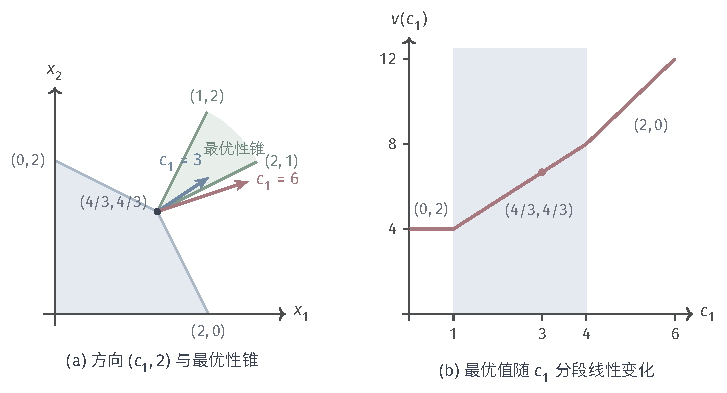
\includegraphics[width=123.126mm]{figures/03-optimization-evolution-and-signals/01-optimization/tikz/c2-cost-sensitivity/figure.pdf}
  \caption{改变第一种产品的获利$c_1$（第二种固定为$2$）。(a) 在顶点$(4/3,4/3)$处，两条活跃约束的外法向$(2,1)$与$(1,2)$张成绿色的最优性锥；目标方向$(c_1,2)$落在锥内时这个顶点最优。蓝色箭头$c_1=3$在锥内，红色箭头$c_1=6$在锥外；$c_1=4$与$c_1=1$恰好对应锥的两条边。(b) 最优获利$v(c_1)$分三段线性变化，各段旁标出最优顶点；浅蓝区域$c_1\in[1,4]$内原基保持最优，斜率为$x_1^\star=4/3$。}
  \label{fig:opt-lp-cost-sensitivity}
\end{figure*}

\paragraph{两种变化的对照}
右端变化与目标系数变化限制原基的方式不同。改变$\bm b$时约化费用不动，原基失效的原因是基本解出现负分量，即原来的顶点已不可行；最优值对$\bm b$的变化率是对偶解$\bm y$，值函数（最大化写法中）是凹的。改变$\bm c$时基本解不动，原基失效的原因是某个约化费用变负，即沿某条边可以改进；最优值对$\bm c$的变化率是原始解$\bm x$，值函数是凸的。两种条件不能互换：资源数量在允许范围内变动时，最优基不变，最优产量却按$\bm A_B^{-1}(\bm b+\Delta\bm b)$移动；产品价格在允许范围内变动时，最优基和最优产量都完全不动，变的只是获利。

\section{线性松弛与原解恢复}
\label{sec:opt-lp-relaxation}

第~\ref{sec:opt-lp-modeling}节看到，产品只能整件生产时，连续模型的解$(4/3,4/3)$不能直接使用。许多离散问题都有类似的结构：候选是有限个点，目标是线性函数。上一节在同一个连续模型内改变数据；本节改变的是问题本身，研究怎样把离散候选放进一个连续的多面体中求解，以及连续解和连续最优值能为原离散问题提供什么。答案分两种情形：若多面体恰好是候选的凸包，最优值不变；若只能用一个更大的多面体，得到的是一个界，原问题的候选还需要另行恢复。

\subsection{精确凸包与线性值保持}
\label{sec:opt-lp-convex-hull}

\paragraph{线性目标在凸包上不变}
设$S\subseteq\mathbb R^d$是非空有限集，目标是线性函数$\bm c^\top\bm x$。凸包$\operatorname{conv}(S)$由$S$中点的全部凸组合组成（见第~\ref{chap:optimization}章），它比$S$大得多，却不会给线性目标带来更好的值。

\begin{theorem}[凸包上的线性值保持]
\label{thm:opt-lp-hull-value}
设$S$是非空有限集。则
\[
  \max_{\bm x\in\operatorname{conv}(S)}\bm c^\top\bm x=\max_{\bm s\in S}\bm c^\top\bm s,
\]
并且$\operatorname{conv}(S)$上的最优解集恰好是$S$中全部最优点的凸包。最小化同理。
\end{theorem}

\begin{proof}
记$M=\max_{\bm s\in S}\bm c^\top\bm s$，有限集上的最大值一定取到。任取$\bm x=\sum_i\lambda_i\bm s_i\in\operatorname{conv}(S)$，$\lambda_i\ge0$，$\sum_i\lambda_i=1$。由线性，
\[
  \bm c^\top\bm x=\sum_i\lambda_i\,\bm c^\top\bm s_i\le\sum_i\lambda_iM=M,
\]
即凸包中任一点的目标值是候选值的加权平均，不超过最大的候选值；而$S\subseteq\operatorname{conv}(S)$，所以两个最大值相等。等号成立当且仅当每个$\lambda_i>0$的$\bm s_i$都满足$\bm c^\top\bm s_i=M$，即$\bm x$只由最优候选组合而成，这给出最优解集的刻画。
\end{proof}

这是线性目标与精确凸包共同给出的结论，两个条件缺一不可。若把目标换成非线性函数，凸组合的目标值不再是加权平均，例如在$S=\{0,1\}$上最大化$x(1-x)$，两个候选的值都是$0$，凸包$[0,1]$上的最大值却在$x=1/2$处取得$1/4$，答案改变了。若把凸包换成一个更大的多面体，最优值一般也会改变，这是下一小节的主题。

\paragraph{最优值保持，输出却可能是分数}
最优值相同，并不意味着在凸包上求解就得到了原问题的解。图~\ref{fig:opt-lp-exact-hull}中$S=\{(0,0),(1,0),(0,1)\}$，在凸包（三角形）上最大化$x_1+x_2$，最优值$1$与原问题相同，但最优面是整条斜边，其中的$(1/2,1/2)$同样最优，却不是原候选。所以“求连续最优值”和“恢复一个原候选”是两个步骤。

\begin{figure}[!htbp]
  \centering
  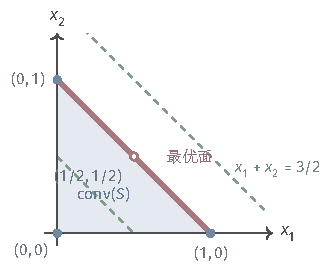
\includegraphics[width=56.257mm]{figures/03-optimization-evolution-and-signals/01-optimization/tikz/c2-exact-hull/figure.pdf}
  \caption{精确凸包上的线性目标。蓝点为三个候选，浅蓝三角形是它们的凸包。最大化$x_1+x_2$的最优值为$1$，与原候选上的最优值相同；红色粗线是最优面，空心点$(1/2,1/2)$在其上，同样最优却不是候选。绿色虚线是值为$1/2$与$3/2$的等值线。}
  \label{fig:opt-lp-exact-hull}
\end{figure}

恢复候选有一条现成的途径。凸包$\operatorname{conv}(S)$的极点都属于$S$：凸包中不属于$S$的点是至少两个不同候选的、系数为正的凸组合，不是极点。若凸包能用有限个线性不等式写出来，单纯形法返回的是基本可行解，即极点（定理~\ref{thm:opt-lp-bfs-extreme}），它自动属于$S$。困难在于前提：对一般的离散问题，凸包的不等式描述可能极为复杂，甚至条数随规模指数增长，无法写出。

网络流是前提成立的重要特例。在第~\ref{sec:opt-lp-reduced-cost}小节对照过的最小费用流中，供需量和容量都是整数时，网络单纯形法的基本可行解在生成树上逐个叶子用守恒式求出，每一步只做整数的加减，所以每个基本可行解都是整数流。线性规划在这里自动给出整数解，依靠的是关联矩阵的特殊结构；一般线性规划没有这一性质，不能期待它的顶点是整数点。

\subsection{外逼近松弛与原解恢复}
\label{sec:opt-lp-outer}

\paragraph{用更大的多面体换取可解性}
写不出精确凸包时，常用的做法是保留原问题中的线性约束，只把“变量取整数”放宽为“变量在区间中”。这样得到的多面体$R$包含全部原候选，但一般比凸包大，称为原问题的\term{线性规划松弛}（linear programming relaxation），也是对凸包的一种\term{外逼近}（outer approximation）。由$S\subseteq R$立即得到：对最大化问题，$\max_R\bm c^\top\bm x\ge\max_S\bm c^\top\bm x$，松弛值是原最优值的上界；对最小化问题，松弛值是下界。

\begin{example}[二元选择]
\label{ex:opt-lp-binary-relaxation}
考虑
\[
  \max\ x_1+x_2\quad\text{s.t.}\quad 2x_1+2x_2\le3,\quad x_1,x_2\in\{0,1\}.
\]
可行候选是$(0,0)$、$(1,0)$、$(0,1)$，$(1,1)$违反约束，所以整数最优值为$1$。把$x_i\in\{0,1\}$放宽为$0\le x_i\le1$，得到图~\ref{fig:opt-lp-outer-relaxation}(a)中的五边形，最优值为$3/2$，在线段$x_1+x_2=3/2$（$1/2\le x_1\le1$）上取得，例如$(3/4,3/4)$与$(1,1/2)$。精确凸包是三角形$x_1+x_2\le1$，五边形比它多出一块。松弛值与原最优值之差$3/2-1=1/2$称为这个实例的加性\term{整数间隙}（integrality gap）；它衡量的是松弛的界偏离了多少，而不是某个算法的误差。
\end{example}

\begin{figure}[!htbp]
  \centering
  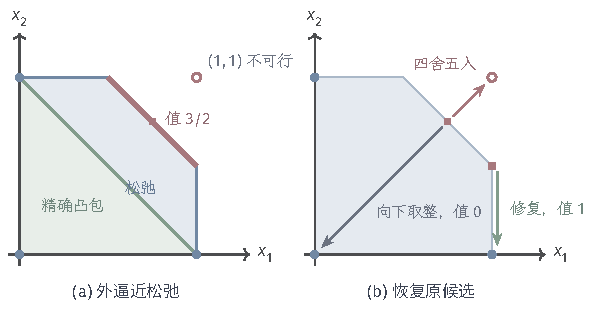
\includegraphics[width=100.986mm]{figures/03-optimization-evolution-and-signals/01-optimization/tikz/c2-outer-relaxation/figure.pdf}
  \caption{二元选择问题的线性规划松弛与候选恢复。(a) 浅蓝五边形是松弛$\{0\le x_i\le1,\ x_1+x_2\le3/2\}$，浅绿三角形是精确凸包；蓝点是可行候选，红圈$(1,1)$违反约束。红色粗线是松弛的最优面，值为$3/2$，红方块$(3/4,3/4)$是其中一点。(b) 三种恢复方式：从$(3/4,3/4)$四舍五入得到不可行的$(1,1)$；向下取整得到可行但值为$0$的$(0,0)$；从$(1,1/2)$把分数坐标降为$0$，得到值为$1$的可行候选$(1,0)$。}
  \label{fig:opt-lp-outer-relaxation}
\end{figure}

\paragraph{从松弛解恢复候选}
松弛给出的点通常不是原候选，需要一个恢复步骤，而恢复后的点要分别检查可行性和目标损失。图~\ref{fig:opt-lp-outer-relaxation}(b)比较了三种做法。若求解器返回$(3/4,3/4)$，四舍五入得到$(1,1)$，违反容量约束；向下取整得到$(0,0)$，可行但获利为$0$，损失了全部收益。若求解器返回顶点$(1,1/2)$，只把唯一的分数坐标降为零，得到$(1,0)$，它满足原约束，获利为$1$。可见恢复规则必须依据原约束设计：对这类“容量不超过”的约束，把变量往下调总能保持可行，但损失多少取决于从哪个松弛解出发、怎样调整。

\paragraph{区间证书}
恢复得到的可行候选与松弛值一起，构成原最优值的一个区间。对最大化问题，可行候选的值是下界，松弛值是上界：二元选择中原最优值落在$[1,3/2]$中。若目标在候选上只取整数，上界还可以向下取整：最优值不超过$\lfloor3/2\rfloor=1$，而$(1,0)$达到$1$，这就证明了$(1,0)$最优。回到章首的作坊：连续松弛值$20/3$说明整件生产的获利不超过$\lfloor20/3\rfloor=6$，而$(2,0)$获利$6$，所以它是整数最优解；把$(4/3,4/3)$向下取整得到的$(1,1)$只获利$5$。

\paragraph{能承诺什么，不能承诺什么}
线性规划松弛是连续问题，可以用单纯形法或第~\ref{chap:constrained-optimization}章的内点法求解，但这并不使离散原问题变得容易：一般的整数线性规划仍是困难问题，松弛只提供一个界和一个恢复的起点。整数间隙可能很大，此时区间证书很宽，恢复出的候选也可能很差；收紧松弛需要加入更多有效不等式，或采用更强的松弛。把变量提升为矩阵、以半正定约束代替线性约束的半正定松弛，留到第~\ref{chap:constrained-optimization}章讨论。

\section{本章小结}
\label{sec:opt-lp-summary}

回到章首的作坊。等值线在可行四边形上平移、最后停在一个角点上，这幅画面在本章变成了一套完整的计算。标准型把各种线性模型统一成$\bm A\bm x=\bm b$、$\bm x\ge\bm 0$；角点是基本可行解，由选定$m$列解一个线性方程组得到；最优值有限时，最优解可以在这有限个基本可行解中找到。单纯形法用约化费用判断哪条边能改进，用最小比值检验决定走多远，从一个基换到相邻的基；两阶段法提供起点，Bland规则排除循环。停止时留下的乘子$\bm y$就是原料的价格：它与最优解同值，证明了最优；第一阶段的乘子在不可行时组合出矛盾；一个可行点加一条下降射线证明无下界。三种结局各有一份不依赖求解过程、只需矩阵乘法就能核对的证书。

本章反复区分了几个容易混淆的结论，它们所需的条件各不相同，表~\ref{tab:opt-lp-summary}把它们放在一起。可行域有界只是最优解存在的充分条件，不是必要条件；线性规划特有的是，只要可行且有下界，最优值就能取到，标准型中还能取在顶点上。有限终止依赖防循环规则和精确算术，它不蕴含多项式时间；数值求解停止、残差很小与严格认证最优是三个不同层次的判断。

\begin{table*}[!htbp]
  \centering
  \caption{本章主要结论及其条件。“标准型”指$\min\bm c^\top\bm x$，$\bm A\bm x=\bm b$，$\bm x\ge\bm 0$；最右列为正文中的位置。}
  \label{tab:opt-lp-summary}
  \begin{tabular}{@{}lll@{}}
    \toprule
    结论 & 所需条件 & 位置 \\
    \midrule
    最优值能取到，且有最优基本可行解 & 标准型可行，目标有下界 & 定理~\ref{thm:opt-lp-optimal-bfs} \\
    基本可行解即极点 & $\bm A$满行秩 & 定理~\ref{thm:opt-lp-bfs-extreme} \\
    约化费用非负推出全局最优 & 当前基可行 & 定理~\ref{thm:opt-lp-optimality-criterion} \\
    单纯形法有限终止 & Bland规则（或其他防循环规则），精确算术 & 定理~\ref{thm:opt-lp-finite} \\
    强对偶，两侧最优解都存在 & 原问题可行且有下界；不需要内点条件 & 定理~\ref{thm:opt-lp-strong-duality} \\
    不可行证书$\bm A^\top\bm z\ge\bm 0$，$\bm b^\top\bm z<0$ & 原约束系统无解 & 定理~\ref{thm:opt-lp-farkas} \\
    无下界证书$(\bm x_0,\bm d)$ & 已知可行点，$\bm A\bm d=\bm 0$，$\bm d\ge\bm 0$，$\bm c^\top\bm d<0$ & 第~\ref{sec:opt-lp-certificates}节 \\
    影子价格给出最优值的变化率 & 右端变化后原基本解仍非负 & 第~\ref{sec:opt-lp-rhs}节 \\
    凸包上线性最优值不变 & 候选集有限，目标线性，凸包精确 & 定理~\ref{thm:opt-lp-hull-value} \\
    \bottomrule
  \end{tabular}
\end{table*}

得到最优解之后的两个问题改变的是不同的对象。参数敏感性仍在同一类连续模型中，回答数据改变时原基还能用多久：右端变化时检查原基本解是否非负，最优值的变化率是影子价格；目标系数变化时检查约化费用是否非负，变化率是原始解。两种情况都只在各自的范围内有效，越过折点就要换基。线性松弛则把另一个离散问题放进连续多面体：精确凸包保持线性最优值，外逼近只给出一个界，恢复原候选还需要依据原约束单独设计，并重新检查可行性。

单纯形法沿可行域的边界从顶点走到顶点。另一条路线是从可行域内部出发，沿一条光滑的路径逼近最优点，这就是内点法。它的每一步需要求解牛顿方程，并借助障碍函数保持在内部，还要处理可行起点与停止依据；这些内容依赖光滑优化的工具，放在第~\ref{chap:constrained-optimization}章集中展开。本章的求解与认证已经由单纯形法和对偶证书完整闭合。

